\documentclass[11pt,a4paper]{article}
\usepackage[margin=25mm]{geometry}
\usepackage{amsmath,amssymb}
\usepackage{graphicx}
\usepackage{booktabs}
\usepackage{array}
\usepackage{xcolor}
\usepackage{float}
\usepackage{caption}
\usepackage[hidelinks]{hyperref}
\usepackage[nameinlink]{cleveref}
\usepackage[autostyle, english = american]{csquotes}
\MakeOuterQuote{"}
\usepackage{microtype}
\emergencystretch=3em
\usepackage{setspace}
\onehalfspacing
\captionsetup{font=small,labelfont=bf}

\newcommand{\bq}[1]{\bar q_{#1}}

\title{Local order parameters for ice polymorphs:\\a unified comparison and practical guide}
\author{Dibyendu Maity\\[2pt]
\small Department of Chemical and Biological Sciences,\\
\small S.~N.~Bose National Centre for Basic Sciences, Salt Lake, Kolkata 700106, India}
\date{}

\begin{document}
\maketitle

\begin{abstract}
Molecular simulations of water and ice rely on local order parameters to tell
solid from liquid, one ice polymorph from another, and to follow nucleation,
growth and interfaces one molecule at a time. Dozens of such parameters have
been proposed, from tetrahedral order and the local structure index to
Steinhardt bond-orientational invariants, CHILL+, template matching and
machine-learned descriptors, but they are usually compared with values taken
from different codes, cutoffs and water models. We review these parameters in
a single taxonomy organized by the structural information they use, and
present a reproducible benchmark of selected parameters for crystalline ice
and supercooled water that asks when they give reliable, transferable
labels: how they survive thermal motion, whether their thresholds transfer
between independent preparations and water models, how they depend on
neighbor conventions, and how much crystal a labeler needs around a molecule.
We compute 22 parameter families (39 scalar outputs) and three labelers with
one open implementation and settings fixed in advance. The main benchmark is
Ih, Ic, stacking-disordered ice and supercooled liquid in TIP4P/Ice at 220~K,
with five independent preparations, extended to TIP4P/2005 and mW, to six
high-pressure ices with pressure-matched liquids, and to constructed seeds;
18 ideal crystal structures serve as a structural reference. Locally averaged
parameters, above all the averaged pair-entropy fingerprint and averaged
$q_6$, separate ice from ambient supercooled liquid almost perfectly, and
averaged $q_3$ and $q_4$ separate hexagonal from cubic ice. In the conditions
tested, their thresholds transfer between independent preparations within
0.003, between protocols and the two TIP4P models within 0.03 and to mW within
0.01, and their scores change by at most 0.025 when the first-shell cutoff is
moved between 3.2 and 3.8~\AA. Distance- and density-based parameters
transfer poorly between models and cutoffs, quenched configurations turn
small density differences into spurious separations, and averaging beyond the
first shell destroys the Ih/Ic signal of $\bar q_3$. Every pair of thermal
high-pressure crystals is separated by some single parameter, but no single
parameter separates every high-pressure ice from liquid at its own pressure,
and none distinguishes proton-ordered from proton-disordered forms of one
oxygen lattice. In constructed seeds, the fraction of molecules assigned the
correct polytype rises with depth below the seed surface; CHILL+ reaches 90\%
at 5--7~\AA{} and PTM about 2~\AA{} deeper, while CHILL+ assigns
many shallower molecules to its interfacial class. We conclude with
recommendations tied to the tested conditions and a reporting checklist.
\end{abstract}

\tableofcontents
\newpage

%=====================================================================
\section{Introduction}\label{sec:intro}
%=====================================================================
Water freezes into more crystalline structures than almost any other simple
substance. Ice Ih, the form of snow and glaciers, is joined by more than twenty
crystalline phases that are stable or metastable at higher pressures, lower
temperatures or both, by several amorphous ices, and by empty and filled
clathrate frameworks~\cite{Salzmann_2019,Hansen2021,Loerting2020}. New phases
are still being found: ice XIX was characterized in
2021~\cite{Gasser2021,Yamane2021}, a metastable ice XXI was obtained from
supercompressed water at room temperature~\cite{Lee2025}, and ice XXII has
been reported above 300~GPa~\cite{Osmond2026}. Molecular simulation is the main
tool for asking how these phases form: how ice nucleates from supercooled
water~\cite{Sosso2016,Sanz2013,HajiAkbari2015,Lupi2017,Piaggi2022}, which
polymorph or stacking sequence grows~\cite{Moore2011,Malkin_2012,Lupi2017},
and how ice behaves at interfaces and in confinement~\cite{Shi2022,Moradzadeh2023}.

Each of these questions requires deciding, for every molecule in every frame,
what kind of local environment it is in. That decision is made with a
\emph{local order parameter} (LOP): a function of the positions of a molecule
and its neighbors that takes characteristic values in each phase. A LOP can do
three different jobs. As a \emph{descriptor} its distribution fingerprints a
phase or a state point. As a \emph{classifier}, with a threshold or a set of
rules, it labels individual molecules, from which nuclei, interfaces and phase
fractions are built. As a \emph{collective variable} (CV) it drives enhanced
sampling, which additionally requires it to be continuous and differentiable
in the coordinates~\cite{Karmakar2021,Neha2022}. Success at one job does not
imply success at another. A parameter whose distributions differ on average
may still misclassify many molecules, and a good classifier may be useless as
a CV.

The choice matters. Computed nucleation barriers and rates from seeding depend
on the order parameter used to measure the nucleus~\cite{Espinosa2016,
SanchezBurgos2022,Gispen2024}, and the size of a nucleus or the width of an
interface changes with the labeling
criterion~\cite{Blow2021,Shi2022}. Popular water order parameters are only
weakly correlated with one another and probe different distortions of the
hydrogen-bond network~\cite{DuboueDijon2015,Donkor2023}. Yet most comparisons
take values from different codes, with different neighbor definitions,
cutoffs, water models and reference structures, so that the parameter cannot
be separated from the way it was computed. Machine-learned classifiers report
accuracies above 99\%~\cite{DeFever2019,Kim2020,Moradzadeh2023}, but on their
own datasets, which makes them hard to compare with each other or with simpler
parameters. Common-setting comparisons do exist: Doi and co-workers screened
493 order parameters and their combinations for Ih, Ic and liquid at
coexistence and for the high-pressure triple points III--V--liquid and
V--VI--liquid~\cite{Doi2021,Doi2021b,Doi2021c}, and Shi and co-workers compared
labelers on the quasi-liquid layer of ice~\cite{Shi2022}. What is less well
established is whether such rankings are reproducible and transferable: how
much of a separation survives thermal motion rather than only energy
minimization, whether a threshold fitted on one trajectory works on an
independently prepared one or on another water model, how strongly results
depend on cutoffs and averaging radii, and how close to an interface a labeler
can still assign the right polytype. These are the questions our benchmark
addresses.

This review has four parts. \Cref{sec:phases} summarizes the ice landscape
and the structural features a local parameter can and cannot see.
\Cref{sec:taxonomy} defines the physically motivated parameters in one
notation, grouped by the information they use, and \cref{sec:ml} reviews
descriptors, learned classifiers and data-driven collective variables.
\Cref{sec:benchmark} reports a reproducible benchmark of selected local
parameters for crystalline ice and supercooled water, in which every
parameter is computed by one open implementation, SolOrder, with settings
fixed before any comparison. It examines thermal robustness, threshold
transferability, neighbor conventions and the spatial limits of local
classification; \cref{tab:coverage} lists exactly what it covers.
\Cref{sec:guide}
turns the results into recommendations and a reporting checklist, and
\cref{sec:outlook} lists open problems.

\paragraph{Scope.} We consider per-molecule parameters for bulk crystalline
ices, empty clathrate frameworks and liquid water, computed from oxygen
positions or full molecular geometries. We do not cover global
crystallographic analysis, spectroscopic observables, electronic structure or
superionic phases. Amorphous ices, machine-learned classifiers and
collective variables are reviewed from the literature but not benchmarked.

%=====================================================================
\section{The ice landscape in brief}\label{sec:phases}
%=====================================================================
\subsection{Phase diagram and stability}
\Cref{fig:phase} shows the experimental phase diagram. Roman numerals now run
to XXII; counting Ih and Ic separately gives more than twenty crystalline
phases~\cite{Salzmann_2019,Hansen2021,Gasser2022,Lee2025,Osmond2026}. Two
caveats apply to any count. The structure of ice XIX is disputed: it was
assigned to a partially antiferroelectric ordering of ice VI in a
$\sqrt2\times\sqrt2\times1$ supercell~\cite{Gasser2021,Yamane2021}, while an
alternative analysis finds HCl-doped ice VI to remain disordered and
distorted~\cite{Salzmann2021b}. And the numeral XXII has been used for two
different structures, a high-pressure orthorhombic phase~\cite{Osmond2026}
and, in a preprint, a metastable phase grown from emulsified water at
250~K~\cite{Kobayashi2025}. Beyond the numbered phases, ice VII becomes plastic
(freely rotating molecules on a bcc lattice) at high temperature, as predicted
by simulation~\cite{Aragones2009} and observed by quasi-elastic neutron
scattering~\cite{Rescigno2025}, and superionic phases form at planetary
conditions~\cite{Millot_2018,Millot2019,Prakapenka_2021,Cheng2021}.

\begin{figure}[H]
\centering
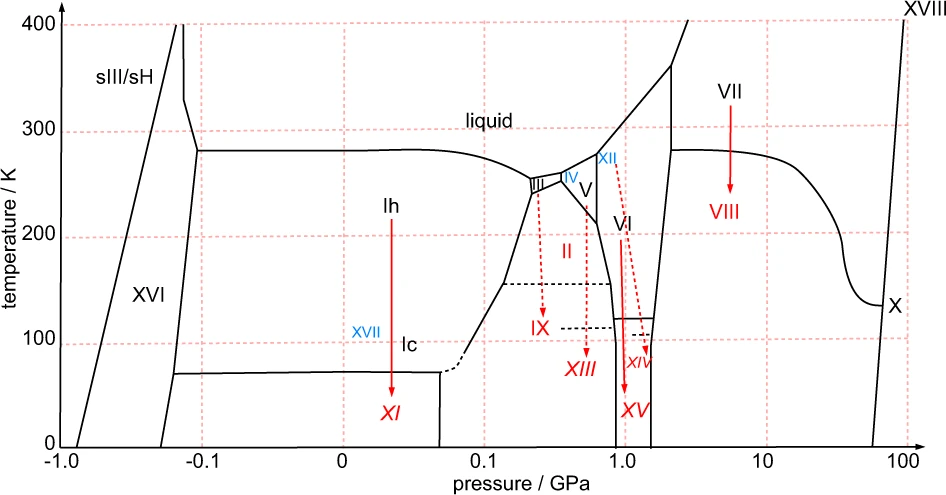
\includegraphics[width=.8\linewidth]{intro/phase.png}
\caption{Experimental phase diagram of water. Black numerals: hydrogen-disordered
phases; red: hydrogen-ordered; blue: metastable. Red arrows mark
order--disorder transitions. Reproduced from Ref.~\cite{Hansen2021} (CC BY 4.0).}
\label{fig:phase}
\end{figure}

Most phases come in pairs. Ih/XI, III/IX, V/XIII, VI/XV, VII/VIII and XII/XIV
share an oxygen framework and differ in whether the protons are ordered; the
ordered form is stable at lower
temperature~\cite{Salzmann_2006,Salzmann_2009,Salzmann_2021}. Stacking adds a
second kind of variety: ice I can stack its puckered layers hexagonally (Ih),
cubically (Ic) or in any mixture, and ice that freezes from supercooled water
is stacking-disordered (Isd) rather than cubic~\cite{Malkin_2012,Malkin2015,
Kuhs2012}. Stacking-disorder-free Ic has been made only indirectly, by
emptying ice XVII or a hydrogen hydrate~\cite{del_Rosso_2020,Komatsu2020}.
Simulated critical nuclei are themselves stacking-disordered~\cite{Lupi2017,
HajiAkbari2015,Niu2019}.

Simulations see the phase diagram of the water model, not that of water.
Rigid nonpolarizable models reproduce its topology to different
degrees~\cite{Sanz2004,Vega2005,Vega2009,Vega2011}. TIP4P/Ice melts at
272.2~K~\cite{Abascal2005a} and its full phase diagram has been mapped with
enhanced sampling~\cite{Bore2022}; TIP4P/2005 melts about 20~K
lower~\cite{Abascal2005b,Conde2017} and its high-pressure diagram includes a
plastic phase~\cite{Aragones2009,Hirata2017}; the oxygen-only mW model melts at
274.6~K~\cite{Molinero2009}. Machine-learned potentials trained on
first-principles data now reproduce the phase diagram
semi-quantitatively, including nuclear quantum
effects~\cite{Cheng2019,Reinhardt2021,Zhang2021,Bore2023,Ibrahim2026}. A state
point that is stable for one model can therefore be metastable, or a
different phase, for another, and every simulation study of ice structure
should state where its state point lies on the model's own phase diagram.

\subsection{Structural signatures relevant to local order}
\Cref{tab:phases} lists, for the phases used in our benchmark, the
quantities a local parameter could exploit, computed from ideal GenIce
structures~\cite{Matsumoto2018,Matsumoto2024}. Three groups stand out. The
low-density, fully tetrahedral frameworks (Ih, Ic, XVII and the clathrates)
have exactly four oxygens within 3.5~\AA{}, near-perfect tetrahedral order $Q$
and a large gap to the fifth neighbor ($d_5\approx4.3$--4.4~\AA). The
intermediate-pressure phases (II, III, V, XII) keep four hydrogen bonds but
fold the network so that non-bonded oxygens enter the first shell: four to six
neighbors within 3.5~\AA, $Q$ of 0.79--0.86 and $d_5$ of 3.2--3.5~\AA. Ice VI
and the VII/VIII family consist of two interpenetrating networks, giving
11--14 neighbors within 3.5~\AA{} and $Q$ as low as 0.33--0.69, even though
every molecule still donates and accepts two hydrogen bonds.

\begin{table}[H]
\centering
\small
\caption{Structural signatures of the crystalline phases in the benchmark.
Density, coordination number (CN, O within 3.5~\AA), mean tetrahedral order
$Q$ and fifth-neighbor distance $d_5$ are computed with SolOrder on ideal
GenIce structures (ice Ic and Ih are shown with the same lattice spacing).
Proton order: D disordered, O ordered; partner: the phase sharing the oxygen
framework.}
\label{tab:phases}
\begin{tabular}{lllcccccc}
\toprule
Phase & Space group & H & Partner & $\rho$ (g\,cm$^{-3}$) & CN & $Q$ & $d_5$ (\AA) \\
\midrule
Ih   & $P6_3/mmc$   & D & XI   & 0.92 & 4.0  & 0.998 & 4.43 \\
Ic   & $Fd\bar3m$   & D & --   & 0.92 & 4.0  & 0.998 & 4.43 \\
II   & $R\bar3$     & O & --   & 1.18 & 5.5  & 0.83  & 3.23 \\
III  & $P4_12_12$   & D & IX   & 1.17 & 4.5  & 0.86  & 3.53 \\
V    & $C2/c$       & D & XIII & 1.24 & 5.8  & 0.80  & 3.32 \\
VI   & $P4_2/nmc$   & D & XV   & 1.37 & 11.5 & 0.69  & 3.36 \\
VII  & $Pn\bar3m$   & D & VIII & 1.60 & 14.0 & 0.40  & 2.90 \\
VIII & $I4_1/amd$   & O & VII  & 1.63 & 13.0 & 0.33  & 2.88 \\
XII  & $I\bar42d$   & D & XIV  & 1.44 & 9.6  & 0.79  & 3.28 \\
XVII & $P6_122$     & D & --   & 0.88 & 4.0  & 0.97  & 4.29 \\
sI (empty) & $Pm\bar3n$ & D & -- & 0.80 & 4.0 & 0.98 & 4.40 \\
\bottomrule
\end{tabular}
\end{table}

What a local parameter cannot see follows from the same table. Proton-order
partners share an oxygen sublattice, so any oxygen-only parameter can
separate them only through the small lattice distortions that accompany
ordering. Ih and Ic have identical first and nearly identical second shells;
they differ in the relative orientation of neighboring tetrahedra (staggered
versus eclipsed bonds) and in the third shell, so a parameter must either
encode bond orientations beyond the first shell or average over neighbors.
Rings are equally uninformative here: both Ih and Ic consist of six-membered
rings only.

\subsection{Amorphous ices, clathrates and liquid water}
Low-density (LDA), high-density (HDA) and very-high-density amorphous ices are
glassy solids whose local structure resembles that of liquids at similar
density~\cite{Loerting2011,AmannWinkel2016,Handle2017,Tonauer2023}, and a
medium-density amorphous ice obtained by ball-milling Ih falls in the gap
between LDA and HDA~\cite{RosuFinsen2023}. Clathrate hydrates build
polyhedral cages from five- and six-membered rings around guest molecules;
their empty frameworks (ices XVI and XVII among them) are tetrahedral like
Ih~\cite{Falenty_2014,del_Rosso_2016}. Supercooled liquid water, finally,
becomes increasingly tetrahedral on cooling and has been described as a
fluctuating mixture of low- and high-density local
structures~\cite{Russo2014,Wikfeldt2011,Tanaka2019,Li2026}; it contains
transient ice-like environments~\cite{Monserrat2020,Capelli2022}. These three
are the hardest cases for local parameters, because they share the
tetrahedral first shell of crystalline ice and differ from it mainly in
medium-range order.

%=====================================================================
\section{A taxonomy of local order parameters}\label{sec:taxonomy}
%=====================================================================
We group physically motivated parameters by the information they use:
distances (radial), angles within the first shell, the hydrogen-bond network,
bond orientations expressed in spherical harmonics, and comparison with a
template. \Cref{tab:taxonomy} summarizes them with the settings used in the
benchmark.

\subsection{Common conventions}
Throughout, $\mathbf r_{ij}=\mathbf r_j-\mathbf r_i$ is the minimum-image
vector between oxygens $i$ and $j$ and $r_{ij}$ its length. Every parameter
needs a neighbor set $N_b(i)$, and the choice is part of the definition:
a radial cutoff (3.5~\AA{} for the first shell of ambient ices, near the first
minimum of $g_{\mathrm{OO}}$), a fixed number of nearest neighbors (four for
tetrahedral parameters), Voronoi neighbors, or hydrogen-bond partners. These
choices give different results~\cite{Mickel2013}, especially at high pressure,
where non-bonded oxygens enter the first coordination shell.
Many parameters exist in a \emph{locally averaged} form,
\begin{equation}
  \bar X(i) = \frac{1}{|N_b(i)|+1} \sum_{j\in\{i\}\cup N_b(i)} X(j),
\end{equation}
introduced for bond-orientational order by Lechner and
Dellago~\cite{Lechner2008} (who average the complex $q_{lm}$ vectors rather
than the scalar, \cref{sec:boo}). Averaging trades spatial resolution for
noise suppression, and as we will see it is the single most important
ingredient at finite temperature. Finally, a parameter used as a CV must be a
continuous, differentiable function of the coordinates. Hard cutoffs, nearest-
neighbor ranks and integer counts are not; switching functions and Gaussian
broadening help, but only if neighbor membership and averaging are smooth
as well.

\subsection{Radial and density-based parameters}
The \emph{coordination number} counts oxygens within $r_c$; its smooth form
replaces the step function with a switching function,
\begin{equation}
  \mathrm{CN}_s(i)=\sum_{j\ne i}\frac{1-(r_{ij}/r_0)^{n}}{1-(r_{ij}/r_0)^{m}},
  \qquad n=12,\ m=28 .
\end{equation}
The \emph{fifth-neighbor distance} $d_5$, the distance to the fifth-nearest
oxygen, measures how far the second shell is from the first and is large in
low-density, tetrahedral environments~\cite{SaikaVoivod2000,Cuthbertson2011}.
The \emph{local structure index}~\cite{Shiratani1996,Shiratani1998} sorts the
distances $r_1<r_2<\dots<r_n<3.7~\AA<r_{n+1}$ and measures the variance of the
gaps $\Delta_k=r_{k+1}-r_k$,
\begin{equation}
  \mathrm{LSI}(i)=\frac1n\sum_{k=1}^{n}\left(\Delta_k-\bar\Delta\right)^2 ,
\end{equation}
which is large when a clear gap separates the first and second shells. The
Voronoi cell of an oxygen gives a local density $1/V$ and a shape measure,
the asphericity $\eta=A^3/(36\pi V^2)$, which is 1 for a sphere and 2.25 for
ice Ih~\cite{Medvedev1989,Ruocco1992,Jedlovszky_1999}. The
\emph{pair-entropy fingerprint}~\cite{Piaggi2017,Piaggi2017b} projects the
two-body excess entropy onto each particle,
\begin{equation}
  s(i)=-2\pi\rho k_B\int_0^{r_m}\left[g_m^i(r)\ln g_m^i(r)-g_m^i(r)+1\right]r^2\,dr,
\end{equation}
where $g_m^i(r)$ is a Gaussian-broadened radial distribution centered on $i$
and $r_m$ is a cutoff of about 5~\AA. Its local average $\bar s$ was designed
as a crystallization CV and uses the whole radial structure out to the second
shell.

\subsection{Angular and tetrahedral parameters}
The \emph{orientational tetrahedral order}~\cite{CHAU_1998,Errington2001},
\begin{equation}
  Q(i)=1-\frac38\sum_{j=1}^{3}\sum_{k=j+1}^{4}\left(\cos\psi_{jik}+\frac13\right)^2,
\end{equation}
uses the angles $\psi_{jik}$ between the four nearest oxygens; it is 1 for a
regular tetrahedron and 0 on average for an ideal gas. The
\emph{translational tetrahedral order}
$S_k=1-\frac13\sum_{k=1}^4(r_k-\bar r)^2/(4\bar r^2)$ measures the variance of
the four nearest distances~\cite{CHAU_1998}. A family of parameters developed
for structure classification by Takahashi, Doi and
co-workers~\cite{Doi2020,Doi2021,Takahashi2023} uses all angles $\theta_{jik}$
in the first shell. The bond-angle parameter averages
$\cos^{n_1}(n_2\theta_{jik}+\phi)$~\cite{Ackland2006,Takahashi2023}; the
angular Fourier series parameter averages
$f(\min(r_{ij},r_{ik}))\cos(a\theta_{jik})$~\cite{Bartk2013,Takahashi2023};
the angle-histogram parameters $H_1$--$H_3$ are Fourier amplitudes of the
histogram of $\theta_{jik}$~\cite{Takahashi2023}; and the common-neighborhood
parameters $A_1$--$A_3$ sum vectors to neighbors shared by $i$ and each of its
neighbors~\cite{Honeycutt1987,Radhi2017,Takahashi2023}.

\subsection{Hydrogen-bond and topology-based parameters}
These parameters need hydrogen positions or a hydrogen-bond network. We use
the geometric criterion of Luzar and Chandler: an O--O distance below
3.5~\AA{} and an H--O$\cdots$O angle below 30$^\circ$~\cite{Luzar1996}.
$N_\mathrm{HB}$ is the number of donated and accepted bonds. The four-body
parameter $F_4=\langle\cos3\phi\rangle$ averages over neighbors the H--O$\cdots$O--H
torsion formed with each molecule's outer hydrogens~\cite{Rodger1996}; it is
about $-0.4$ in ice, $-0.04$ in the liquid and $0.7$ in clathrate
hydrates~\cite{Rodger1996,Jimnezngeles2014}. The selection of the outer
hydrogen matters: choosing it per molecule from the opposite oxygen is the
correct form, and we found and fixed an implementation that did otherwise.
The Russo--Tanaka $\zeta$ is the distance to the nearest non-hydrogen-bonded
oxygen minus that to the farthest hydrogen-bonded one~\cite{Russo2014}; it
is positive in locally favored, tetrahedral structures. Ring statistics count
the smallest rings of the hydrogen-bond network passing through each
molecule~\cite{King1967,Franzblau1991,Matsumoto2007}. Different ring
definitions give different results~\cite{Formanek2020}, and in small periodic
cells paths that wrap around the box must be rejected, or they are counted as
rings.

\subsection{Bond-orientational order}\label{sec:boo}
Steinhardt parameters~\cite{Steinhardt1983} expand the directions to the
neighbors in spherical harmonics,
\begin{equation}
  q_{lm}(i)=\frac{1}{|N_b(i)|}\sum_{j\in N_b(i)}Y_{lm}(\hat{\mathbf r}_{ij}),\qquad
  q_l(i)=\sqrt{\frac{4\pi}{2l+1}\sum_{m=-l}^{l}|q_{lm}(i)|^2},
\end{equation}
and build the third-order invariant
$w_l=\sum_{m_1+m_2+m_3=0}\begin{pmatrix}l&l&l\\m_1&m_2&m_3\end{pmatrix}q_{lm_1}q_{lm_2}q_{lm_3}$
and its normalized form $\hat w_l=w_l/(\sum_m|q_{lm}|^2)^{3/2}$. Lechner and
Dellago average the vectors,
$\bar q_{lm}(i)=\sum_{j\in\{i\}\cup N_b(i)}q_{lm}(j)/(|N_b(i)|+1)$, and form
$\bar q_l$ from them~\cite{Lechner2008}; this picks up the orientation of the
second shell. Odd $l$ matter for water: $l=3$ captures tetrahedral symmetry,
and $\bar q_3$ and $\bar q_4$ distinguish Ih from Ic~\cite{Benet2014,Doi2021}.
The ten Wolde--Frenkel \emph{crystalline connections} count neighbors $j$ with
normalized dot product $\mathbf q_6(i)\cdot\mathbf q_6(j)>0.5$~\cite{tenWolde1996}.
For water, Reinhardt and co-workers designed Steinhardt-based parameters able
to drive ice growth~\cite{Reinhardt2012}, Haji-Akbari and Debenedetti
labeled molecules with $q_6>0.5$ within 3.2~\AA{} in their direct
nucleation-rate calculation~\cite{HajiAkbari2015}, and seeding studies tune a
$\bar q_6$ threshold by a mislabeling criterion~\cite{Espinosa2016}.

The CHILL algorithm~\cite{Moore2010} uses the correlation
$c(i,j)=\mathbf q_3(i)\cdot\mathbf q_3(j)/(|\mathbf q_3(i)||\mathbf q_3(j)|)$
for each bond to the four nearest neighbors. Bonds with $c<-0.8$ are
staggered and bonds with $-0.2<c<-0.05$ eclipsed; four staggered bonds mean
cubic ice and three staggered plus one eclipsed hexagonal ice, with further
rules for interfacial ice. CHILL+~\cite{Nguyen2014} widens the eclipsed window
to $-0.35<c<0.25$, uses neighbors within 3.5~\AA, and adds clathrate classes
for molecules with four eclipsed bonds. It was designed to detect hexagonal
ice up to its melting point.

\subsection{Template and symmetry-based parameters}
The centrosymmetry parameter sums $|\mathbf r_{ij}+\mathbf r_{ik}|^2$ over
opposite pairs of the 12 nearest neighbors and vanishes for a centrosymmetric
environment~\cite{Kelchner1998}. The neighbor-distance parameter $D$ averages
products of functions of the three distances in each neighbor
triangle~\cite{Takahashi2023}. Polyhedral template matching (PTM) finds the
template (here hexagonal or cubic diamond) with the lowest root-mean-square
deviation after optimal rotation and scaling, and accepts it below an RMSD
cutoff~\cite{Larsen2016}; the related identify-diamond method uses common
neighbor analysis of the second shell~\cite{Maras2016,Stukowski2012}. The
local-order metric of Martelli and co-workers measures the best overlap of a
neighborhood with a reference lattice~\cite{Martelli2018,Martelli2018b}.

\subsection{Other recent parameters}
Several recent parameters are not in our benchmark: an O--O--O--O dihedral
parameter that separates Ih, Ic and high- and low-density liquid with Bayesian
classification~\cite{Matsumoto2019}, the hydrogen-bond-network indicator
$\Psi$~\cite{Foffi2024}, and an environment-similarity CV for oxygen-only ice
growth~\cite{Piaggi2020}. Supervised screens over hundreds of candidate
parameters and their combinations~\cite{Doi2020,Doi2021,Doi2021b,Doi2021c,
Takahashi2023b} and graph-network-designed parameters~\cite{Ishiai2023} have
also produced task-specific sets.

\subsection{Summary table}
\Cref{tab:taxonomy} lists every parameter in the benchmark with the settings
used there. "Smooth form" marks a parameter defined through a switching
function or Gaussian broadening. In our implementation neither marked
parameter is a tested CV: both are truncated at the 5~\AA{} search cutoff
(where the switching function is small but not zero) and use hard neighbor
membership.

\begin{table}[H]
\centering
\footnotesize
\caption{Local order parameters in the benchmark, with the settings used
there. All O--O first-shell cutoffs are 3.5~\AA. H: needs hydrogen positions.}
\label{tab:taxonomy}
\begin{tabular}{>{\raggedright\arraybackslash}p{.24\linewidth}>{\raggedright\arraybackslash}p{.11\linewidth}>{\raggedright\arraybackslash}p{.28\linewidth}cc>{\raggedright\arraybackslash}p{.12\linewidth}}
\toprule
Parameter & Group & Neighbors & H & \begin{tabular}[b]{@{}c@{}}Smooth\\form\end{tabular} & Ref. \\
\midrule
CN & radial & O within 3.5~\AA & & & -- \\
Smooth CN & radial & switching function, $r_0=3.5$~\AA & & \checkmark & -- \\
$d_5$ & radial & fifth-nearest O & & & \cite{Cuthbertson2011} \\
LSI & radial & O within 3.7~\AA{} and next & & & \cite{Shiratani1996} \\
Voronoi density, asphericity & radial & periodic Voronoi cell & & & \cite{Medvedev1989,Ruocco1992} \\
Entropy $s$, $\bar s$ & radial & $g(r)$ to 5~\AA; average to 5~\AA & & \checkmark & \cite{Piaggi2017,Piaggi2017b} \\
$Q$, $\bar Q$ & angular & 4 nearest O; average 3.5~\AA & & & \cite{Errington2001} \\
$S_k$ & angular & 4 nearest O & & & \cite{CHAU_1998} \\
Bond angle $B$ & angular & O within 3.5~\AA & & & \cite{Ackland2006,Takahashi2023} \\
Angular Fourier ($a=3$) & angular & O within 3.5~\AA & & & \cite{Bartk2013,Takahashi2023} \\
Angle histogram $H_1$--$H_3$ & angular & O within 3.5~\AA & & & \cite{Takahashi2023} \\
$A_1$--$A_3$ & angular & O within 3.5~\AA & & & \cite{Radhi2017,Takahashi2023} \\
$F_4$ & H-bond & O within 3.5~\AA, outer H & \checkmark & & \cite{Rodger1996} \\
$N_\mathrm{HB}$ & H-bond & 3.5~\AA, 30$^\circ$ & \checkmark & & \cite{Luzar1996} \\
$\zeta$ & H-bond & H-bond partners; O to 5~\AA & \checkmark & & \cite{Russo2014} \\
Ring fractions (4--8), mean & H-bond & H-bond network, rings $\le 10$ & \checkmark & & \cite{King1967,Franzblau1991} \\
$q_3$, $q_4$, $q_6$ & bond-orient. & O within 3.5~\AA & & & \cite{Steinhardt1983} \\
$\bar q_3$, $\bar q_4$, $\bar q_6$ & bond-orient. & averaged over 3.5~\AA & & & \cite{Lechner2008} \\
$\hat w_4$, $\hat w_6$ & bond-orient. & O within 3.5~\AA & & & \cite{Steinhardt1983} \\
Crystalline connections & bond-orient. & $\mathbf q_6$ dot product $>0.5$ & & & \cite{tenWolde1996} \\
Centrosymmetry & template & 12 nearest O & & & \cite{Kelchner1998} \\
Neighbor distance $D$ & template & O within 3.5~\AA & & & \cite{Takahashi2023} \\
CHILL / CHILL+ & labeler & 4 nearest / 3.5~\AA, $\mathbf q_3$ & & & \cite{Moore2010,Nguyen2014} \\
PTM & labeler & diamond templates, RMSD $<0.1$ & & & \cite{Larsen2016} \\
\bottomrule
\end{tabular}
\end{table}

%=====================================================================
\section{Descriptors and machine-learned approaches}\label{sec:ml}
%=====================================================================
\subsection{High-dimensional descriptors}
Machine-learning methods replace one scalar with a vector that describes the
whole neighborhood. A useful descriptor is invariant to translation, rotation
and permutation of identical atoms, changes smoothly with the coordinates,
is complete enough to distinguish different environments, and is cheap to
compute~\cite{Musil2021,Langer2022}. Atom-centered symmetry functions sum
radial and angular terms over neighbors~\cite{Behler2011}. The smooth overlap
of atomic positions (SOAP) expands a Gaussian-smeared neighbor density in
radial functions and spherical harmonics and forms the rotationally invariant
power spectrum $p_{nn'l}=\sum_m c_{nlm}c_{n'lm}$~\cite{Bartk2013,Willatt2019};
Steinhardt $q_l$ is closely related to it, retaining
a single radial channel~\cite{Musil2021}. Many-body tensor representations encode distributions
of distances and angles~\cite{Huo2022}. Libraries such as
DScribe~\cite{Himanen2020} make these descriptors easy to compute. For water,
SOAP shows that the liquid contains local environments resembling a wide range
of ice phases~\cite{Monserrat2020}, that classical rigid models contain
short-lived ice-like environments~\cite{Capelli2022}, and that SOAP and
standard order parameters do not tell the same story about the
liquid~\cite{OffeiDanso2022,Donkor2023}.

\subsection{Supervised classifiers}
Supervised networks are trained on molecules of known phase. Geiger and
Dellago trained a neural network on symmetry functions to identify liquid and
several ice phases~\cite{Geiger2013}. DeepIce feeds the Cartesian coordinates
of the nearest neighbors to a deep network and was applied to ice surfaces,
where it outperformed Steinhardt, tetrahedral and template
labels~\cite{Fulford2019}. A PointNet-based network reached 99.1\% accuracy
over liquid, five ice phases and sI and sII hydrates using oxygen positions
alone, about 99.6\% with hydrogens, with most errors between sI and sII; with
interfacial molecules included its accuracy fell to about
92\%~\cite{DeFever2019}. GCIceNet, a graph convolutional network on the
hydrogen-bond graph with order parameters as node features, reported 99.8\%
test accuracy over nine TIP4P/Ice classes~\cite{Kim2020}, and an
edge-conditioned graph network 99.9\% over nine phases, including the
interface and water in nanotubes~\cite{Moradzadeh2023}. Score-based denoising
can first remove thermal noise and then classify with simple
parameters~\cite{Sun2024}, and a variational autoencoder on SOAP features
identifies ice phases without labels in its latent space~\cite{Maity2025}.

These accuracies are not directly comparable. Each refers to its own classes,
water model, temperature and train/test split; most test molecules come from
the same trajectories as the training molecules; and accuracy on bulk phases
says little about interfaces, which is where the classification matters most.
The benchmark in \cref{sec:benchmark} shows that, with averaging, simple
scalars already separate ambient ice from liquid with more than 99\% balanced
accuracy on held-out runs, so a learned model has to be judged on harder
tasks: interfaces, high-pressure ice against dense liquid, and transfer to
other water models.

\subsection{Unsupervised approaches}
Unsupervised methods look for structure in descriptor space without labels.
Autoencoders and Gaussian mixtures on bond-order parameters recover
crystalline and hidden local structures in colloidal
systems~\cite{Boattini2019,Boattini2020}; persistent-homology descriptors with
clustering follow nucleation in metals~\cite{Becker2022b,Becker2022}; and a
generalized convex hull with sketch-map projection organized nearly
75,000 hypothetical ice structures derived from zeolite networks and
recovered the known phases among them~\cite{Engel2018}. Near the
liquid--liquid critical point of a water model, local descriptors show no
two-state structure while non-local ones reveal low- and high-density
domains~\cite{Donkor2024}. Unsupervised maps are descriptive. Turning a
cluster into a phase label still requires reference structures, and the
clusters depend on the descriptor and its cutoffs.

\subsection{Data-driven collective variables}
Enhanced sampling of nucleation needs a CV that is differentiable and that
follows the slow structural change. Hand-built CVs for ice include
Steinhardt-based parameters~\cite{Quigley2008,Reinhardt2012}, the averaged
pair entropy~\cite{Piaggi2017b}, an environment-similarity
kernel~\cite{Piaggi2020}, and combinations tuned for
crystallization~\cite{Zhang2019,Niu2019}. Data-driven CVs learn a
low-dimensional combination of many descriptors, by discriminant analysis
between basins (Deep-LDA)~\cite{Bonati2020} or by the slowest modes of a
biased trajectory (Deep-TICA)~\cite{Bonati2021}, and are typically combined
with OPES~\cite{Invernizzi2020}. The mlcolvar library exports such models to
PLUMED~\cite{Bonati2023}. Graph neural networks can learn nucleation CVs from
Steinhardt features~\cite{Dietrich2024} or directly from
coordinates~\cite{Zhang2024}, although neither has yet been tested on ice. In
parallel, machine-learned potentials of first-principles
quality~\cite{Zhang2018,Babin2013,Babin2014,Medders2014,Schran2021} have
brought nucleation studies to ab initio accuracy~\cite{Cheng2018,Niu2020,
Piaggi2022,Piaggi2024}; they all still rely on a local order parameter to
define the nucleus.

%=====================================================================
\section{A unified benchmark}\label{sec:benchmark}
%=====================================================================
All parameters in \cref{tab:taxonomy} were computed with one implementation
(SolOrder, MIT license), one set of settings fixed before any comparison, and
one analysis pipeline. Differences between parameters therefore reflect the
parameters, not codes or cutoffs; the effect of the water model was measured
separately. Before the benchmark, every parameter was checked against
independent references: q$_l$ against the Legendre addition formula (to
$2\times10^{-15}$), direct geometric formulas for tetrahedral, radial and LSI
parameters, MDAnalysis torsions for $F_4$, OVITO for CHILL+ (exact agreement
on all GenIce phases tested), and serial against parallel execution on 366
frames from 44 nucleation trajectories.

\subsection{Datasets}\label{sec:datasets}
\paragraph{Ideal crystals.} Eighteen structures were generated with
GenIce2~\cite{Matsumoto2018,Matsumoto2024}: Ih, Ic, II, III, IV, V, VI, VII,
VIII, IX, XI, XII, XIII, XIV and XVII, and the empty sI, sII and sH clathrate
frameworks. Each proton-disordered phase was generated from five random
seeds (89,100 molecular environments). Ice XVI was excluded because GenIce
gives it the same oxygen positions as the empty sII framework. Every atom was
displaced by Gaussian noise of 0.02~\AA, about twice the coordinate precision
of the files, so that two phases count as separable only at a stated
resolution. Five pairs are proton order--disorder partners: Ih/XI, III/IX,
V/XIII, VII/VIII and XII/XIV.

\paragraph{Seed test (run A).} Bulk Ih, Ic and stacking-disordered ice, and
spherical Ih, Ic and stacking-disordered seeds of 50, 100 and 200 molecules
in liquid, were simulated with TIP4P/Ice~\cite{Abascal2005a} at 220~K at
constant volume. Each of the twelve systems contributes ten thermal frames
and the same frames after energy minimization (834,040 environments). Every
molecule carries a label from the construction: seed membership, depth below
the seed surface, and hexagonal or cubic stacking of its layer. The liquid
reference consists of molecules more than 8~\AA{} beyond the seed radius.

\paragraph{Replicas (run B) and independent preparations (runs C1--C5).} Run
B repeats bulk Ih, Ic, stacking-disordered ice and liquid (4096 molecules) at
220~K, and Ih and Ic at 250~K, from the same structures, with 60 frames 5~ps
apart (1,643,520 environments). Runs C1--C5 start from new structures: Ih and
Ic get new proton configurations, generated by ice-rule loop
moves~\cite{Rick2003,Buch1998} with the net dipole below 2\% of full
polarization; stacking-disordered ice gets a new random stacking sequence;
each liquid is remelted at 300~K and re-equilibrated for 1~ns at 220~K
(8,217,600 environments). Crystal oxygens stay within 0.35--0.41~\AA{} of
their minimized sites. The 220~K liquid is slow (about 3~\AA{} per ns) and
still aging slightly, but CHILL+ labels about 10\% of its molecules as ice or
interfacial ice with no trend.

\paragraph{Water models (run D).} TIP4P/2005~\cite{Abascal2005b} was run on
the C1--C3 structures at 220~K (the same temperature) and at 200~K (about the
same undercooling), together with a TIP4P/Ice control under the same
protocol, so that moving a threshold from run C to the control measures the
protocol effect and moving it from the control to TIP4P/2005 the model effect.
Each system was equilibrated at 1~bar (anisotropic Monte Carlo barostat for
crystals) and then sampled at constant volume (9,953,280 environments). The
oxygen-only mW model~\cite{Molinero2009}, implemented in OpenMM~\cite{Eastman2024}
and checked against an independent energy calculation to $3\times10^{-15}$,
was run on the C1--C3 oxygen positions at 220~K, close to the TIP4P/Ice
undercooling (3,548,160 environments). Ih densities are 0.925 (TIP4P/2005),
0.912 (TIP4P/Ice) and 0.979~g\,cm$^{-3}$ (mW).

\paragraph{High-pressure phases (run E).} Ices II and III at 0.3~GPa, V at
0.5~GPa, VI at 1.0~GPa, and VII and VIII at 3.0~GPa were generated with GenIce2
(two seeds, every periodic height at least 24~\AA), and liquid at each of
these pressures (0.3, 0.5, 1.0 and 3.0~GPa) from the 4096-molecule liquid,
remelted at 300~K and the target pressure, all with TIP4P/Ice at 220~K. Crystals
were equilibrated for 200~ps at pressure (flexible barostat for the
triclinic cells) and sampled as above (5,432,640 environments). All phases
were retained: oxygens moved 0.25--0.45~\AA{} over 300~ps, and the mean cosine
between each molecule's dipole direction at the first and last frame stayed
at 0.96, including the proton-ordered II and VIII. Densities were 1.18 (II),
1.15 (III), 1.26 (V), 1.35 (VI), 1.56 (VII) and 1.57~g\,cm$^{-3}$ (VIII). Ice
VII is metastable relative to VIII at 220~K and stays disordered only because
rigid-water simulations do not order protons on this time scale.

Every thermal frame has a matching energy-minimized (quenched) frame, which
removes thermal vibration while keeping the structure. \Cref{tab:coverage}
summarizes the coverage and the role of each dataset. The benchmark contains
about $3.0\times10^7$ molecular environments, but that number measures
computational coverage, not evidence: molecules in one frame, and frames of
one trajectory, are strongly correlated. The inferential weight rests on the
independent units, which are five preparations for the ambient phases at
220~K, three per water model and two per high-pressure phase.

\begin{table}[H]
\centering
\footnotesize
\caption{Coverage of the benchmark. Prep.: independent preparations (new
proton configurations, stacking sequences or remelted liquids). Frames: thermal
frames per run, each with a quenched copy. Everything not listed, including
amorphous ices, thermal clathrates, ices IV, IX and XI--XVII at finite
temperature, three-site water models and other temperatures and pressures, is
outside the benchmark.}
\label{tab:coverage}
\setlength{\tabcolsep}{3pt}
\begin{tabular}{>{\raggedright\arraybackslash}p{.11\linewidth}>{\raggedright\arraybackslash}p{.21\linewidth}>{\raggedright\arraybackslash}p{.15\linewidth}>{\raggedright\arraybackslash}p{.14\linewidth}cc>{\raggedright\arraybackslash}p{.14\linewidth}}
\toprule
Dataset & Phases & Model & $T$, $P$ & Prep. & Frames & Role \\
\midrule
Ideal & 18 GenIce structures & none & -- & 5 seeds$^a$ & 1 & structural reference \\
Run A & bulk Ih, Ic, Isd; seeds of 50--200 molecules in liquid & TIP4P/Ice & 220~K, 1~bar & 1 & 10, 1~ps & interface depth, labelers \\
Run B & Ih, Ic, Isd, liquid & TIP4P/Ice & 220~K (Ih, Ic also 250~K), 1~bar & 1$^b$ & 60, 5~ps & held-out transfer \\
C1--C5 & Ih, Ic, Isd, liquid & TIP4P/Ice & 220~K (Ih, Ic also 250~K), 1~bar & 5 & 60, 5~ps & main benchmark \\
Run D & Ih, Ic, Isd, liquid & TIP4P/2005; TIP4P/Ice NPT control; mW & 220~K (TIP4P/2005 also 200~K$^c$), 1~bar & 3 & 60, 5~ps & model and protocol transfer \\
Run E & II, III, V, VI, VII, VIII; liquid at each pressure & TIP4P/Ice & 220~K, 0.3--3.0~GPa & 2 & 60, 5~ps & high-pressure extension \\
Sensitivity & Ih, Ic, liquid (C1--C3) & TIP4P/Ice & 220~K, 1~bar & 3 & 12, 25~ps & neighbor conventions \\
Nucleation & 44 trajectories & TIP4P/Ice, mW & various & -- & 366 total & qualitative application \\
\bottomrule
\end{tabular}

\raggedright\footnotesize $^a$ For proton-disordered phases; ordered phases
repeat. $^b$ Same starting structures as run A. $^c$ Ih, Ic and liquid.
\end{table}

\subsection{Separability metric}
For a scalar parameter and two populations $A$ and $B$ we use the two-sample
Kolmogorov--Smirnov statistic
$D_{AB}=\sup_x|F_A(x)-F_B(x)|$, where $F_A$ and $F_B$ are the empirical
cumulative distributions over the molecules of each population. $D$ needs no
binning, which matters for the near-delta distributions of ideal crystals, and
$(1+D)/2$ is exactly the balanced accuracy of the best single threshold
chosen on the same data. We report it as an \emph{oracle score}, between 0.5
(no separation) and 1 (perfect separation). Because the threshold is
optimized on the evaluated molecules, it is not a predictive accuracy. We
therefore also report \emph{held-out} scores: the balanced accuracy of a
threshold and direction fitted on one run and applied to another, with
missing values counted as errors. Molecules within one frame are correlated,
so bootstrap intervals resample frames (blocks of five frames, 25~ps, in run
B) rather than molecules. Such intervals describe variation within one
trajectory and are therefore narrow; the spread between independent
preparations is the better measure of uncertainty and is the one we quote.
Labelers (CHILL, CHILL+, PTM) are scored against the construction labels.

\subsection{Ideal crystals}
Of the 153 pairs of ideal crystals, 150 are separated at an oracle score of
at least 0.95 by at least one parameter (\cref{fig:sep-ideal}). The three
exceptions are Ih/XI (best 0.87, smooth CN), V/XIII (best 0.83, $\bar q_4$)
and sI/sII (best 0.92). The first two are proton order--disorder partners
whose oxygen frameworks barely differ, and no hydrogen-aware parameter
($F_4$, $\zeta$, $N_\mathrm{HB}$, ring fractions) separates them either. The
other partner pairs are separable only because GenIce's ordered cells are
slightly distorted: III/IX by $\bar s$ alone, VII/VIII by 17 parameters and
XII/XIV by five. The most broadly useful parameters are $\bar s$ (93\% of
pairs at 0.95 or above), Voronoi asphericity (90\%), Voronoi density and
$\bar Q$ (89\%). $N_\mathrm{HB}$ separates no pair, because every molecule in
every ideal crystal has four hydrogen bonds; $A_3$ separates none either.

\begin{figure}[H]
\centering
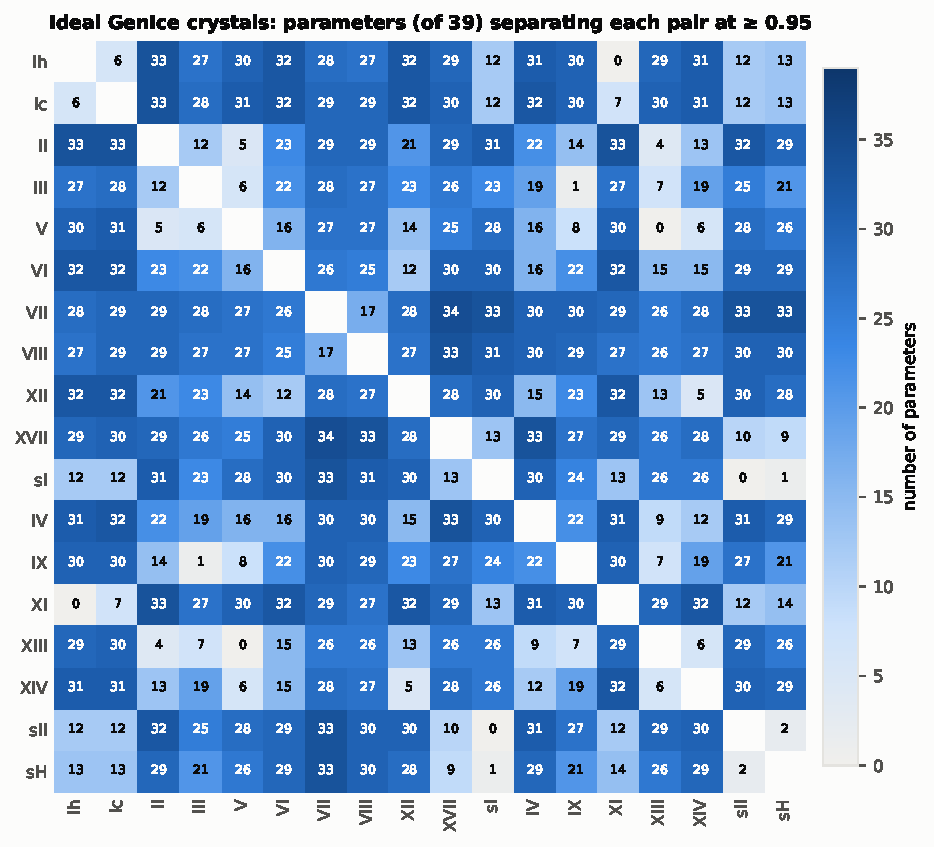
\includegraphics[width=.8\linewidth]{../benchmarks/results/figures/F1a_separability_ideal.pdf}
\caption{Number of parameters (of 39) that separate each pair of ideal
crystals with an oracle score of at least 0.95.}
\label{fig:sep-ideal}
\end{figure}

\subsection{Thermal motion: averaging is what survives}
At 220~K the picture changes (\cref{fig:sep-thermal}). For ice against
liquid, the best parameters are locally averaged: $\bar s$ (1.00), $\bar q_6$
(0.99) and $\bar Q$ (0.98), compared with 0.85, 0.78 and 0.84 for their
unaveraged forms. The six-ring fraction (0.99) is the best unaveraged
parameter, since ring statistics already span several molecules. The cutoff
coordination number (0.62) and $N_\mathrm{HB}$ (0.53) are nearly useless:
supercooled liquid water is almost fully four-coordinated and hydrogen-bonded.
Energy minimization restores most of the separation removed by thermal
motion: $d_5$, LSI and $\zeta$ rise from 0.83--0.84 to 1.00.

Hexagonal and cubic ice are separated at 220~K only by $\bar q_3$ (1.00),
$\bar q_4$ (1.00), $F_4$ (0.94), crystalline connections (0.93), $\bar q_6$
(0.78) and centrosymmetry (0.72); every other parameter is at 0.61 or below,
including ring statistics, which cannot distinguish them. $\bar s$ separates
Ih from Ic perfectly in ideal crystals but only at 0.61 at 220~K. At 250~K
the order is unchanged ($\bar q_3$ 1.00, $\bar q_4$ 0.99, $F_4$ 0.91,
crystalline connections 0.88). These results agree with earlier findings that
$\bar q_4$ separates Ih from Ic at the ice--water interface~\cite{Benet2014}
and that low-$l$ averaged parameters are the best pair in a supervised
screen~\cite{Doi2021}.

\begin{figure}[H]
\centering
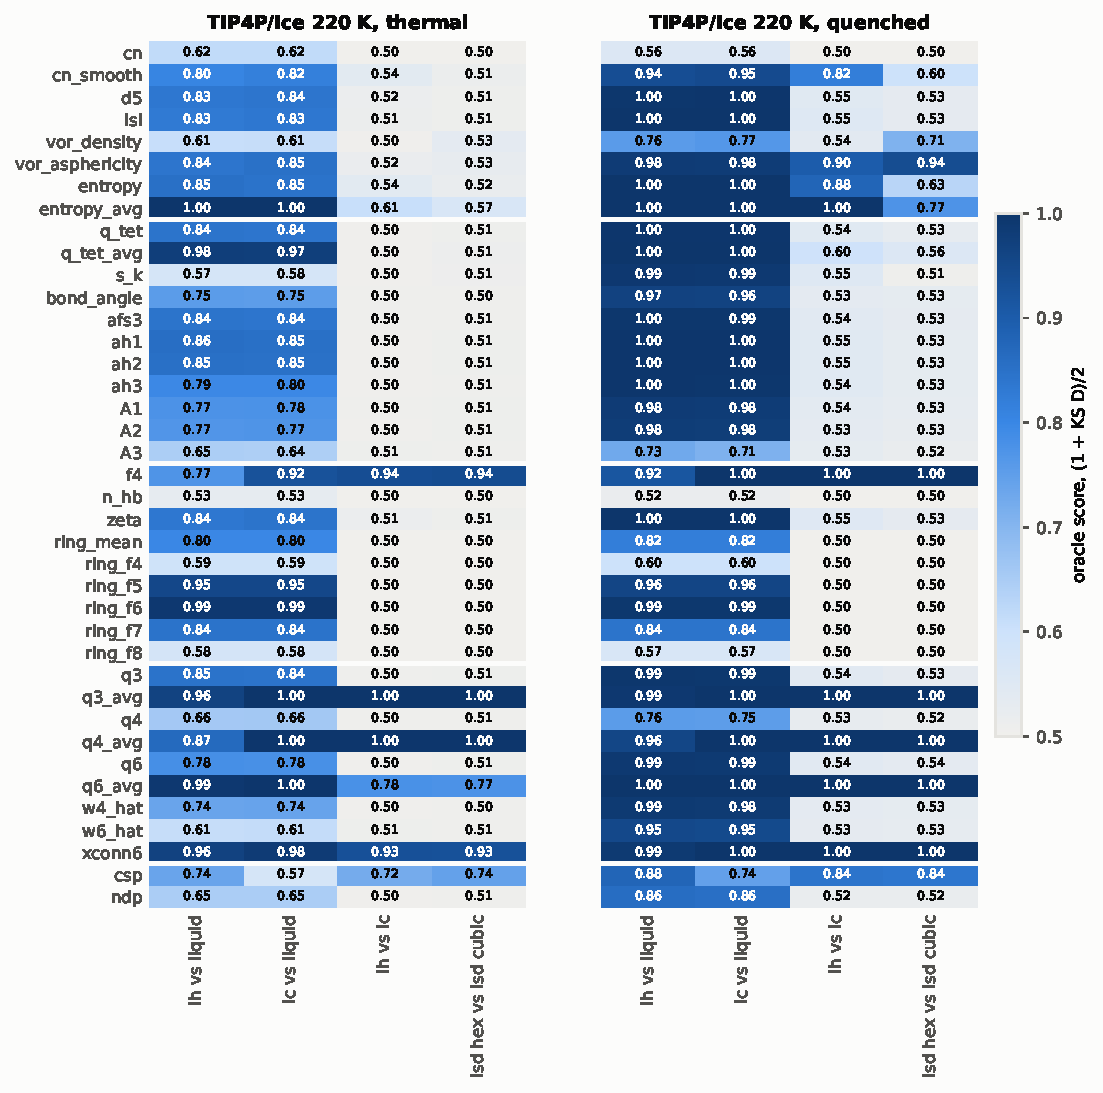
\includegraphics[width=.95\linewidth]{../benchmarks/results/figures/F1b_separability_thermal.pdf}
\caption{Oracle score $(1+D)/2$ for ice versus liquid, Ih versus Ic, and
hexagonal versus cubic layers in stacking-disordered ice, TIP4P/Ice at 220~K.
Left: thermal frames; right: the same frames after energy minimization.}
\label{fig:sep-thermal}
\end{figure}

Many parameters carry nearly the same information in these data. Grouping
parameters whose Spearman rank correlation, pooled over thermal Ih, Ic and
liquid at 220~K, exceeds 0.8 in absolute value reduces the 39 columns to 22
groups (\cref{fig:redundancy}). The largest joins $Q$, the bond angle, the
angular Fourier term, the three angle-histogram amplitudes, $q_3$, $q_6$ and
$\hat w_4$: in this mixture of ambient ice and liquid they rank molecules
almost identically. Pooled correlations largely reflect the ice--liquid
contrast, so they show redundancy for that task, not equivalence in general,
and need not hold for other phases or conditions. Other groups join $\bar q_3$, $\bar q_4$, $\bar q_6$ and
crystalline connections; $d_5$, LSI, $s$ and $\zeta$; $\bar Q$ and $\bar s$;
and the five- and six-ring fractions.

\begin{figure}[H]
\centering
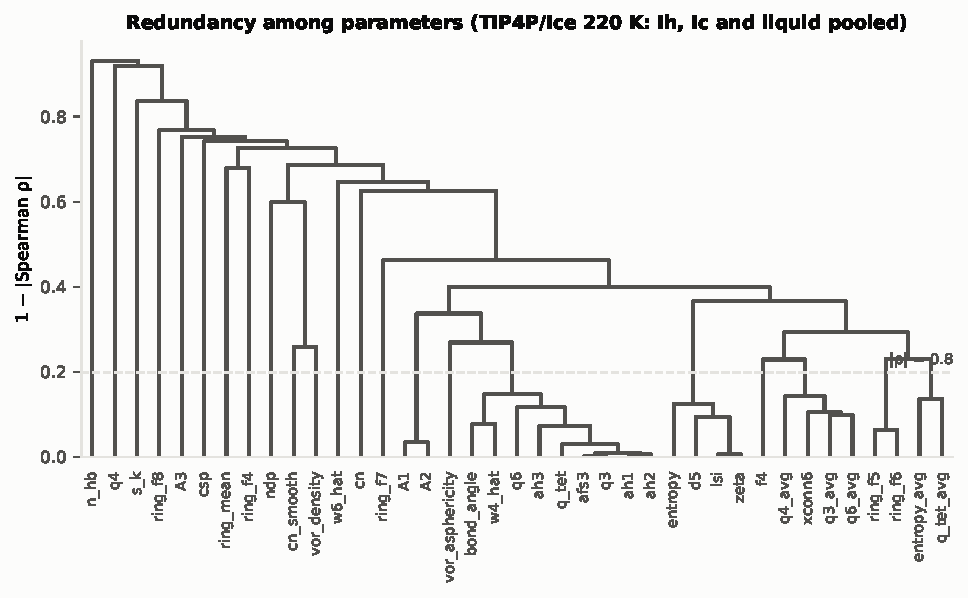
\includegraphics[width=.9\linewidth]{../benchmarks/results/figures/F2_redundancy.pdf}
\caption{Hierarchical clustering of parameters by $1-|\rho|$, with $\rho$ the
Spearman correlation over thermal Ih, Ic and liquid molecules at 220~K. The
dashed line marks $|\rho| = 0.8$.}
\label{fig:redundancy}
\end{figure}

\subsection{How far do thresholds transfer?}\label{sec:transfer}
\paragraph{Between runs and preparations.} A threshold and direction fitted on
run A and applied to run B lose at most 0.008 in balanced accuracy relative
to the oracle score on run B, for every parameter and population pair,
thermal or quenched (\cref{fig:heldout}). With $10^4$--$10^5$ molecules per
population a single threshold barely overfits, and the best parameter for
each task is the same under both scores. Across the five independent
preparations the median standard deviation of the oracle score is 0.001;
wherever the mean oracle score is at least 0.8, leaving one preparation out
costs at most 0.001 and thresholds fitted on run A cost at most 0.003
(\cref{fig:grouped}). Hydrogen-aware parameters score within 0.009 of each
other in the polarized run A crystals and the unpolarized preparations.
Weak separations are another matter. In quenched stacking-disordered ice,
smooth CN separates hexagonal from cubic layers at 0.60 in one preparation
but 0.51--0.52 in the other four, and a threshold fitted on four preparations
scores 0.45 on the fifth: the stacking sequence, not the parameter, produced
the separation. In these data, every separation that failed to reproduce
across preparations was below about 0.65. We use that value as an empirical
warning for these datasets, not as a general reliability threshold.

What matters more than the run is which populations are compared. With the
bulk liquid of run B instead of the far liquid around the seeds of run A, 25
of 156 ice/liquid scores change by more than 0.01, all of them distance- or
density-based (CN, smooth CN, $d_5$, Voronoi, bond angle, $A_1$, $A_2$,
centrosymmetry, $D$), by up to 0.05.

\begin{figure}[H]
\centering
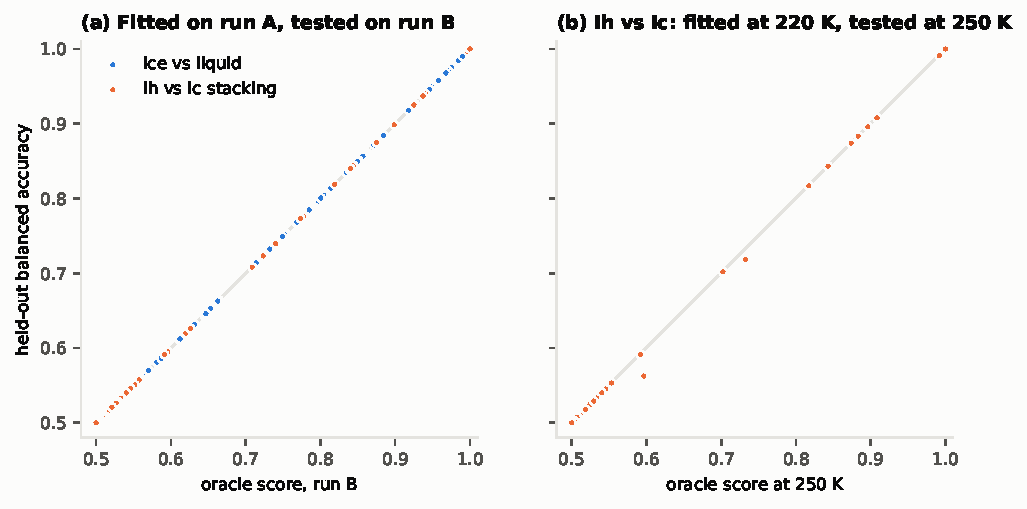
\includegraphics[width=.9\linewidth]{../benchmarks/results/figures/S2_heldout.pdf}
\caption{Held-out against oracle scores, one point per parameter and
population pair (thermal and quenched). (a) Threshold fitted on run~A,
balanced accuracy on run~B, at 220~K. (b) Ih versus Ic in run~B: threshold
fitted at 220~K, balanced accuracy at 250~K.}
\label{fig:heldout}
\end{figure}

\begin{figure}[H]
\centering
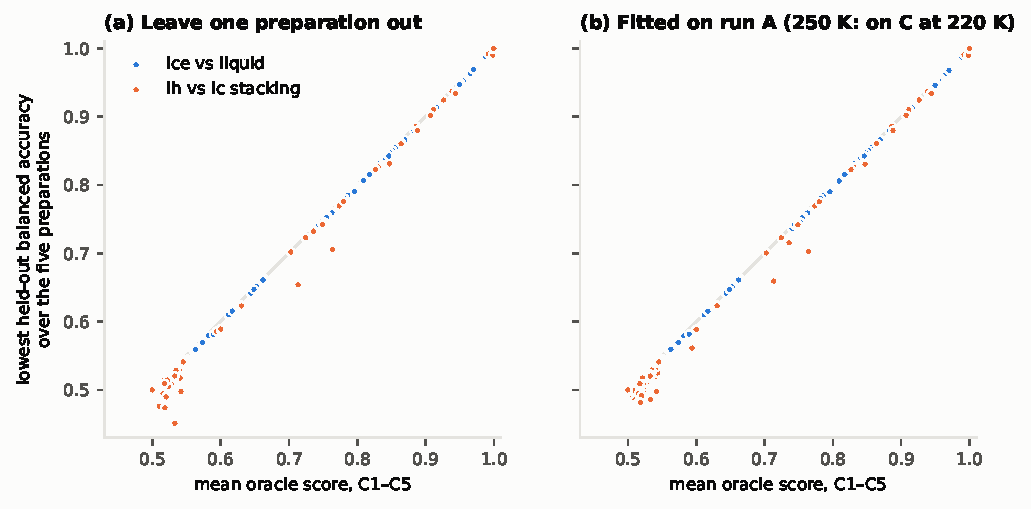
\includegraphics[width=.9\linewidth]{../benchmarks/results/figures/S3_grouped.pdf}
\caption{Five independent preparations (C1--C5). Vertical axis: lowest
held-out balanced accuracy over the five preparations, for a threshold fitted
(a) on the other four preparations and (b) on run~A.}
\label{fig:grouped}
\end{figure}

\paragraph{Between water models.} Thermal frames transfer between the two
TIP4P models (\cref{fig:model}a--c). From TIP4P/Ice to TIP4P/2005, oracle
scores change by a median 0.004 (at most 0.025) at the same temperature or the
same undercooling, and wherever the oracle score is at least 0.8 a threshold
fitted on TIP4P/Ice loses at most 0.033 on the worst TIP4P/2005 preparation.
Changing the protocol from the constructed constant-volume box to NPT costs at
most 0.012. Quenched frames are the exception: their distributions are so
narrow that the best threshold sits at a model-specific value. Smooth CN and
Voronoi density keep oracle scores of 0.97 and 0.82 for ice versus liquid in
either model, but thresholds moved from TIP4P/Ice score only 0.47--0.65 on
TIP4P/2005.

The oxygen-only mW model is a harder test (\cref{fig:model}d). The leading
parameters still transfer within 0.01: $\bar s$ (1.000), $\bar q_6$ (0.998),
$\bar Q$ (0.991) and $\bar q_3$ (0.987) for ice versus liquid, $\bar q_3$ and
$\bar q_4$ (at least 0.998) for Ih versus Ic. First-shell distance parameters,
however, fail to transfer even in thermal frames, because the mW liquid packs
more neighbors into the first shell (median smooth CN 4.76, against 4.39 for
TIP4P/Ice). Smooth CN separates ice from mW liquid with an oracle score of
0.90 but scores 0.67 with the TIP4P/Ice threshold; $A_1$ drops from 0.80 to
0.72 and $d_5$ and LSI lose about 0.04.

\paragraph{Density artifacts in quenched frames.} The narrowness of quenched
distributions also turns small density differences into spurious structure.
Under NPT, Ic comes out 0.35\% denser than Ih in both TIP4P models, and that
alone gives Voronoi density and $D$ oracle scores of 0.74--0.90 for quenched
Ih versus Ic, against 0.52--0.55 in a fixed box. In mW, with no proton
disorder to blur the lattice, quenched Ih and Ic are separated almost
perfectly (at least 0.998) by smooth CN, Voronoi density and asphericity,
entropy and $D$. Neither is a stacking signal; both are lattice-parameter
signals.

\begin{figure}[H]
\centering
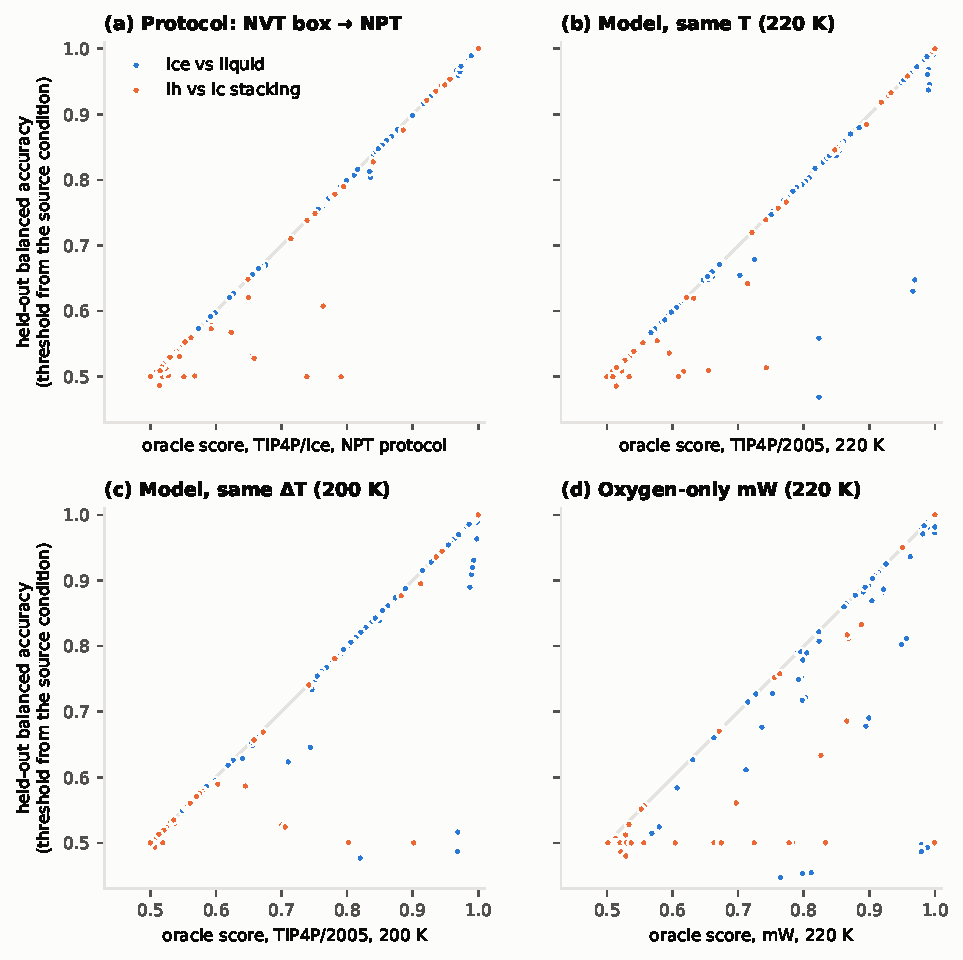
\includegraphics[width=\linewidth]{../benchmarks/results/figures/S4_model.pdf}
\caption{Moving thresholds between protocols and water models. Horizontal
axis: oracle score on the target condition; vertical axis: held-out score of
the threshold fitted on the source condition. (a) TIP4P/Ice, constant-volume
box to NPT protocol. (b, c) TIP4P/Ice to TIP4P/2005 at 220~K and at 200~K.
(d) TIP4P/Ice to mW at 220~K; hydrogen-dependent parameters are absent. The
outliers far below the diagonal are distance- and density-based parameters,
in quenched frames for TIP4P/2005 and also in thermal frames for mW.}
\label{fig:model}
\end{figure}

\subsection{High-pressure phases}\label{sec:pressure}
Every pair of the eight thermal crystals (Ih, Ic, II, III, V, VI, VII, VIII)
is still separated by some single parameter (\cref{fig:pressure}a): the best
held-out score, taking the worse of the two preparations, is at least 0.98
for every pair except VII/VIII, where $\bar q_6$ reaches 0.92 (1.00 in
quenched frames, through the angle histogram). Individual parameters suffer
much more than this best case (\cref{fig:pressure}b). Of the 684 crystal pair
and parameter combinations with an ideal oracle score of at least 0.95, 31\%
fall below 0.95 and 10\% below 0.8 in thermal frames; quenching restores all
but 3.5\%. Losses are largest for $\hat w_4$ and $\hat w_6$ (median
0.23--0.26), $D$ (0.14), and unaveraged $q_6$, $F_4$ and entropy
(0.06--0.08), and near zero for averaged and network parameters. $\bar s$
separates crystal pairs best on average (mean held-out 0.96), followed by
smooth CN, Voronoi asphericity and $\bar Q$ (0.94).

Because the crystals were sampled at different pressures, a comparison of
ice with liquid at another pressure mixes structure with state point. We
therefore ran liquid at the pressure of every crystal and treat the
pressure-matched pairs as the test of ice-versus-liquid identification; the
other pairs measure discrimination among the sampled phase and state-point
combinations. At 3.0~GPa and 220~K the liquid is nearly arrested (oxygens
move 0.5~\AA{} in 300~ps, compared with 2~\AA{} at 0.3--0.5~GPa) and stays
amorphous, with a density of 1.44~g\,cm$^{-3}$ against 1.56 for ice VII, so it
is closer to a compressed glass than to a liquid.

Matched against liquid at its own pressure, with the worse held-out score of
the two preparations, ice VI (1.00, $\bar s$), VII and VIII (1.00, $\bar s$)
are separated perfectly, II reaches 0.97 (six-ring fraction), III 0.95
($\bar s$) and V only 0.84 ($\bar q_4$). Quenching raises V to 0.93. Ice V,
with its 28-molecule cell and wide range of local environments, is the one
phase that no single local parameter separates from liquid at its own
pressure. No single parameter covers all matched pairs: the best worst case
is $\bar Q$ at 0.69 (0.65 over all ice and liquid pairs). Liquids are hard to
tell apart from each other at nearby pressures (0.64 between 0.3 and 0.5~GPa,
0.75 between 0.5 and 1.0~GPa, best with smooth CN). Ice-versus-liquid choices
made at ambient pressure therefore do not carry over, and pairwise separation
by one threshold does not imply that one classifier would sort all these
phases at once.
Thresholds are also fragile in quenched high-pressure frames: of the crystal
pair and parameter combinations above, 62 quenched scores of at least 0.8 lose
more than 0.02 between the two preparations (none in thermal frames), mostly for ices II and VIII. Quenched
ordered crystals have nearly delta-shaped distributions ($d_5$ standard
deviation 0.0002--0.003~\AA), and the two preparations differ by their final
box (0.4\% in density for ice II), which moves the peaks by more than their
width.

\begin{figure}[H]
\centering
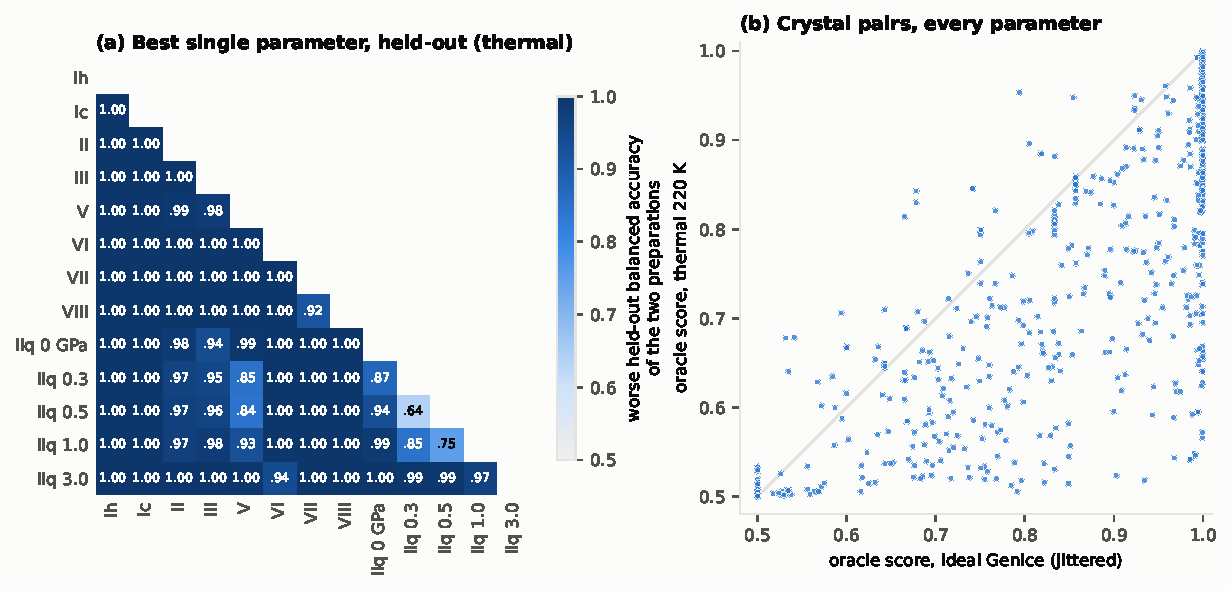
\includegraphics[width=\linewidth]{../benchmarks/results/figures/F8_pressure.pdf}
\caption{Thermal high-pressure phases, TIP4P/Ice at 220~K. (a) Best single
parameter per pair, scored by the worse of the two held-out directions
between preparations; liquid at the pressure of each crystal (0, 0.3, 0.5,
1.0 and 3.0~GPa; the 3.0~GPa liquid is nearly arrested). (b) Every parameter and
crystal pair: oracle score of the ideal, jittered GenIce structures against
the thermal oracle score.}
\label{fig:pressure}
\end{figure}

\subsection{Polytype recall against depth in constructed seeds}
This section asks a narrower question than "does a labeler recognize ice":
for molecules of a constructed Ih, Ic or stacking-disordered seed in
TIP4P/Ice liquid at 220~K, how often does a labeler assign the bulk polytype
of the molecule's layer, and how does that depend on the molecule's depth
below the seed surface? A molecule that is not assigned the correct polytype
can instead be assigned the wrong polytype, an interfacial-ice class (CHILL
and CHILL+ only) or no ice class at all; these are different outcomes, and we
report them separately. Each seed is one trajectory with ten frames 1~ps
apart, so the intervals below describe variation within that trajectory.

In bulk ice, CHILL+ labels 99.7\% of thermal Ih correctly, the original CHILL only
70.7\%. The eclipsed-bond window explains the difference. In thermal bulk Ih
every four-coordinated molecule keeps its three staggered bonds, but the
correlation of its eclipsed bond falls inside CHILL's window $(-0.2,-0.05)$
for only 70.8\% of molecules (5th--95th percentile $-0.23$ to $0.01$),
against 100\% for the CHILL+ window $(-0.35,0.25)$. After energy minimization
both windows contain every eclipsed bond. This quantifies the improvement
CHILL+ was designed for~\cite{Nguyen2014}. PTM with the default RMSD cutoff
labels 97\% of bulk ice correctly and never labels liquid as ice.
False-positive rates in the far liquid are at most 1\% for all three
labelers.

In the seeds all three recover only part of the constructed crystal
(\cref{fig:labels}): CHILL+ finds 11\% of the interior molecules of a
50-molecule Ih seed with the correct polytype, and 58\% for a 200-molecule
seed. Construction labels describe the starting structure, so we audited each
frame before reading these numbers as errors. A seed molecule counts as intact
when it lies within 1~\AA{} of its constructed site (after removing the
seed's drift) and keeps all its constructed bonds shorter than 3.5~\AA. In the
100- and 200-molecule seeds 81--90\% of seed molecules are intact (94--99\% of
interior ones); the 50-molecule Ih seed is the most deformed, 57\% intact.

\begin{figure}[H]
\centering
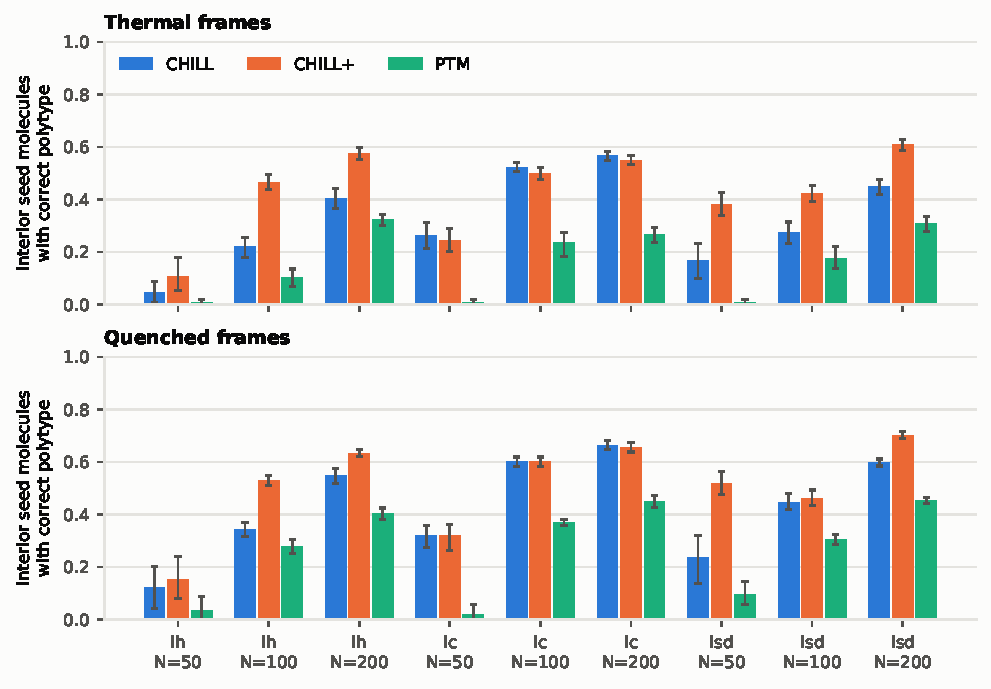
\includegraphics[width=.85\linewidth]{../benchmarks/results/figures/F7_seed_labels.pdf}
\caption{Fraction of interior seed molecules labeled with the correct
polytype by CHILL, CHILL+ and PTM, for Ih, Ic and stacking-disordered (Isd)
seeds of $N$ molecules in TIP4P/Ice liquid at 220~K. Error bars: 95\%
bootstrap intervals over the ten frames of one trajectory per seed (1~ps
apart); they do not include variation between independent seeds.}
\label{fig:labels}
\end{figure}

Polytype recall depends on depth below the constructed seed surface and
hardly on seed size (\cref{fig:depth}), but the three labelers behave
differently. \emph{CHILL+} assigns the correct polytype to at most 15\% of
molecules within 3~\AA{} of the surface, 68--80\% at 4--5~\AA{} and at least
90\% from 5--6~\AA{} (Ic, stacking-disordered) or 6--7~\AA{} (Ih), although
about 90\% of molecules are intact already at 2--4~\AA. Most of the rest near
the surface is not misassigned: at 3--4~\AA{} it puts 44--47\% of molecules in
its interfacial-ice class, 15--25\% in no ice class, and at most 7\% in the
wrong polytype. \emph{CHILL} behaves like CHILL+ for Ic seeds, but for Ih and
stacking-disordered seeds its recall stays at 0.5--0.9 even deep inside,
the same eclipsed-window deficit as in bulk Ih. \emph{PTM} has no
interfacial class and never assigns the wrong polytype; it needs about 2~\AA{}
more depth than CHILL+, reaching 50--55\% at 5--6~\AA{} and 82--90\% at
6--8~\AA. A 50-molecule seed (radius about 7.3~\AA) has only 3--4\% of its
molecules deeper than 5~\AA, which explains most of its low score.
Small-seed recall therefore measures how much crystalline support a labeler
needs before it assigns a bulk polytype, not whether it detects ice; with its
interfacial class, CHILL+ detects some form of ice at much smaller depths.
The depths quoted hold for these constructed seeds in TIP4P/Ice at 220~K. This is
consistent with the observation that labelers disagree mainly at
interfaces~\cite{Shi2022}, and it bears directly on nucleus sizes from
seeding, which depend on where the labeler places the
surface~\cite{Espinosa2016,SanchezBurgos2022,Gispen2024}.

\begin{figure}[H]
\centering
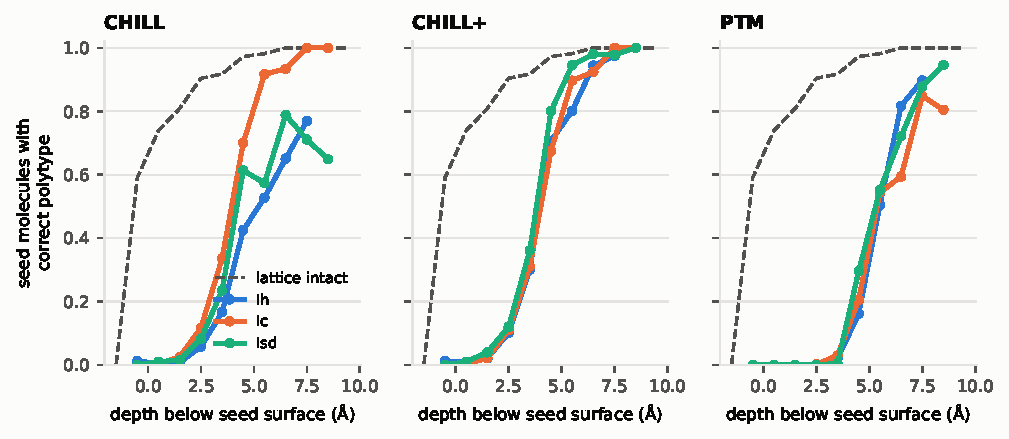
\includegraphics[width=.85\linewidth]{../benchmarks/results/figures/F7b_seed_depth.pdf}
\caption{Polytype recall against depth: fraction of seed molecules labeled
with the correct polytype against depth below the constructed seed surface,
pooled over seed sizes, thermal frames at 220~K; molecules deeper than about
9~\AA{} come only from the 200-molecule seeds. Dashed: fraction of molecules whose constructed lattice is
intact. Bins with fewer than 30 molecules are omitted.}
\label{fig:depth}
\end{figure}

\subsection{Application: nuclei along nucleation paths}
As a qualitative check outside the benchmark data, we computed all parameters
on 366 frames from 44 nucleation trajectories (biased path sampling,
metadynamics, shooting and brute-force runs, TIP4P/Ice and mW). In the 34
frames of four fixed-box TIP4P/Ice path-sampling trajectories whose largest
connected CHILL+ ice core holds at least 20 molecules, we compared each
parameter with membership of that core. The median ROC area under the curve
is highest for $\bar q_6$ (0.985), followed by $\bar Q$ and $\bar q_3$ (0.97),
$\bar s$ (0.96, lower inside the core), crystalline connections (0.95) and
$\bar q_4$ (0.93); $N_\mathrm{HB}$ is near 0.5. The ranking matches the bulk
benchmark. Because CHILL+ is itself built from $\mathbf q_3$ correlations,
this is agreement with a reference labeler, not independent accuracy, and the
biased paths give no rates.

\subsection{Sensitivity to the neighbor convention}\label{sec:sensitivity}
All results above use the registry defaults. To see how much they depend on
that choice, we varied one factor at a time on preparations C1--C3 at 220~K
(bulk Ih, bulk Ic and liquid, 12 thermal frames 25~ps apart and their quenched
counterparts; 571,392 environments): the first-shell cutoff of every
cutoff-based parameter and of CHILL and CHILL+ from 3.2 to 3.8~\AA, the LSI
shell radius over the same range, the averaging radius of $\bar q_l$ and
$\bar Q$ from 3.2 to 5.0~\AA{} with $q_{lm}$ and $Q$ kept at 3.5~\AA, and the
integration radius $r_m$ of the pair entropy, which in our implementation is
also its averaging radius, from 4.0 to 6.0~\AA. Rank-based parameters ($d_5$,
$Q$, $S_k$, centrosymmetry) and Voronoi parameters have no cutoff. Besides the
oracle score we fitted a threshold on C1 at the default setting and applied it
to C2 and C3 computed with the varied setting, which is what happens when a
published threshold is reused with a different convention
(\cref{fig:sensitivity}).

\paragraph{First-shell cutoff.} The leading parameters barely notice it. For
thermal Ih versus liquid, $\bar q_6$ stays at 0.987--0.992 and the six-ring
fraction at 0.989--0.992; for Ih versus Ic, $\bar q_3$ stays at 0.983--1.000,
$\bar q_4$ at 0.993--0.997, $F_4$ at 0.930--0.939 and crystalline connections
at 0.906--0.925, all lowest at 3.8~\AA. Their thresholds fitted at 3.5~\AA{}
lose at most 0.025 at any other cutoff. The ranking of the 30 scanned columns
is stable (Spearman correlation with the default ranking at least 0.94 for
ice versus liquid and 0.99 for Ih versus Ic), and the three best parameters
for Ih versus Ic are the same at every cutoff. Unaveraged first-shell
parameters are another story. For thermal Ih versus liquid, 15 of the 30
columns change by more than 0.02, all of them rising with the cutoff: CN from
0.53 to 0.81, smooth CN from 0.63 to 0.87, $D$ from 0.57 to 0.76, the
bond-angle parameter from 0.73 to 0.85 and $A_1$ from 0.76 to 0.87. A larger
cutoff reaches the interstitial molecules that distinguish the liquid, so
none of these parameters has a natural cutoff, and published values computed
with different cutoffs cannot be compared. Smooth CN is the extreme case: its
threshold fitted with $r_0=3.5$~\AA{} scores only 0.50--0.69 at any other $r_0$.
Hydrogen-bond parameters ($N_\mathrm{HB}$, $\zeta$, ring fractions) and the LSI
shell radius hardly matter (LSI 0.832--0.834), because the angular part of the
hydrogen-bond criterion, not the distance, decides which pairs count.

\paragraph{Averaging radius.} Averaging further than the first shell
improves the even-$l$ parameters: for thermal Ih versus liquid, $\bar Q$ rises
from 0.976 to 1.000 and $\bar q_4$ from 0.870 to 0.923 at 5~\AA, and for Ih
versus Ic $\bar q_6$ rises from 0.776 to 0.962. $\bar q_3$ does the opposite.
Its perfect Ih/Ic separation exists only with first-shell averaging and falls
to 0.894, 0.647 and 0.804 at averaging radii of 4.0, 4.5 and 5.0~\AA. The
$\mathbf q_3$ vectors of neighboring molecules in a tetrahedral network are
anti-correlated (the staggered bonds of CHILL), so the average depends on how
many molecules of each sublattice it contains, and the second shell adds them
in a different proportion. Thresholds of $\bar q_3$, and of $\bar q_4$ for ice
versus liquid, do not survive a change of averaging radius at all (0.50).

\paragraph{Entropy radius.} $\bar s$ separates thermal ice from liquid at 0.95
with $r_m=4$~\AA{} and 1.00 from 5~\AA{} on; it never separates thermal Ih from
Ic (at most 0.63). In quenched frames it separates Ih from Ic perfectly at the
default $r_m=5.0$~\AA{} but only at 0.53--0.77 at any other radius: the
integration limit happens to fall where the sharp quenched radial
distributions of the two polytypes differ. The perfect quenched separation in
\cref{fig:sep-thermal} is an accident of the cutoff, not a property of the
parameter. Thresholds of $s$ and $\bar s$ are tied to $r_m$ (0.50 when it
changes).

\paragraph{Labelers.} CHILL+ labels 99.7\% of thermal bulk Ih correctly with
cutoffs of 3.3--3.5~\AA, 98.6\% at 3.7~\AA{} and 96.1\% at 3.8~\AA, because it
labels only molecules with exactly four neighbors inside the cutoff. CHILL
uses the four nearest neighbors and is insensitive to the cutoff (70.7--71.0\%
for Ih, at least 99.3\% for Ic). Both keep false positives in the liquid
below 1\% at every cutoff.

\begin{figure}[H]
\centering
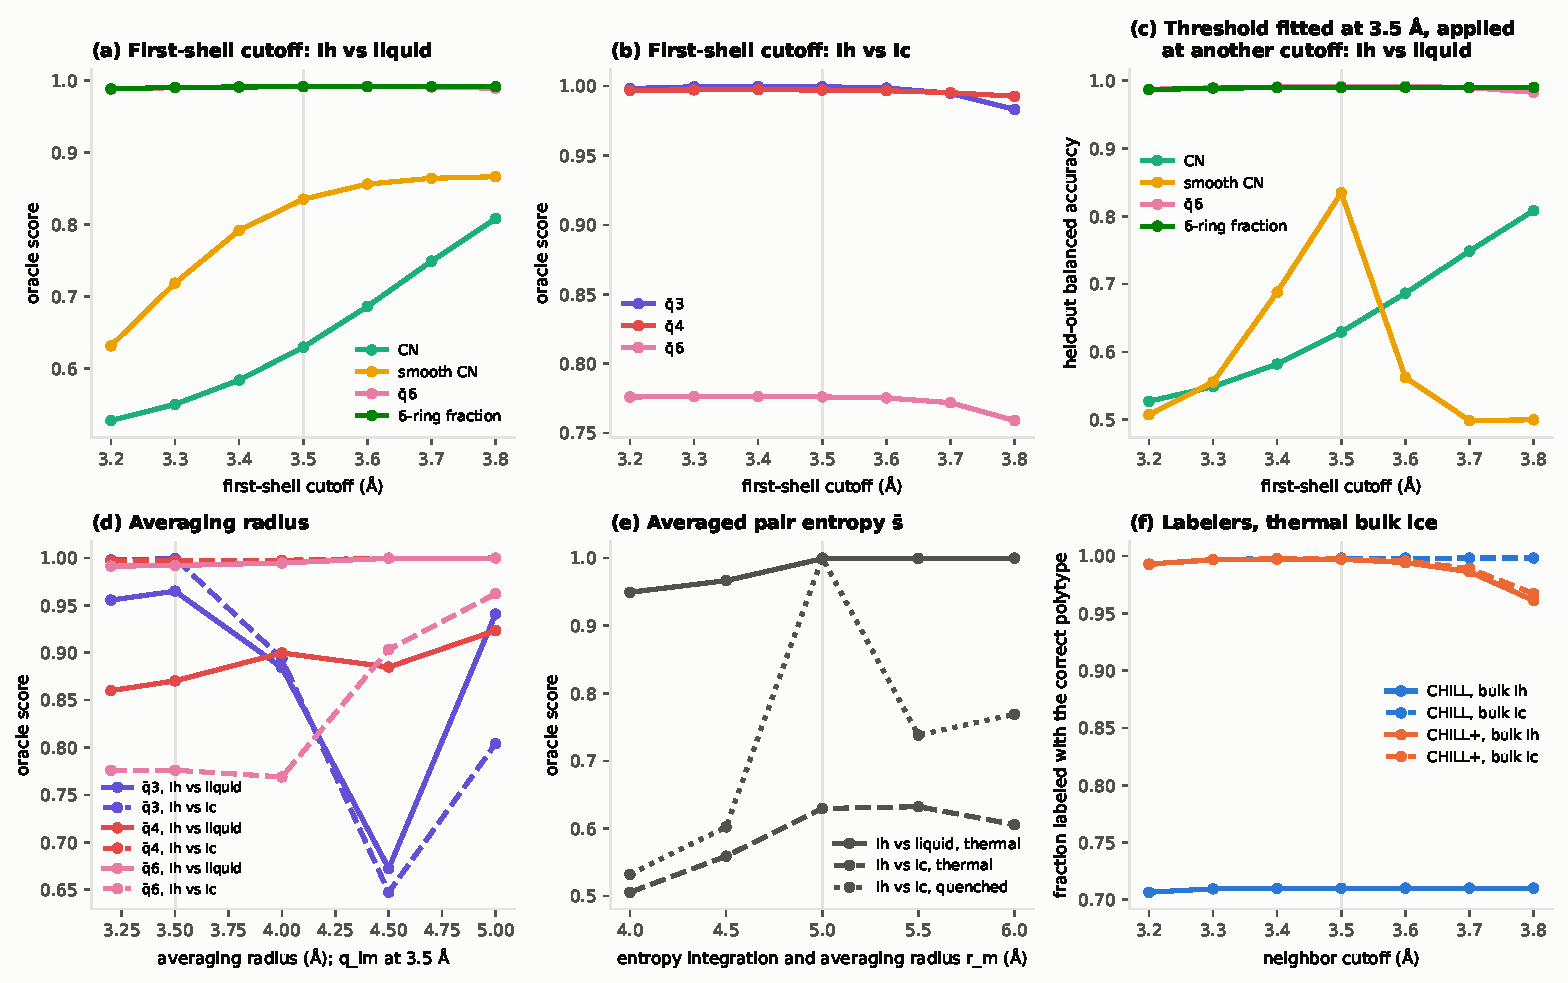
\includegraphics[width=\linewidth]{../benchmarks/results/figures/F5_sensitivity.pdf}
\caption{Sensitivity to the neighbor convention, run C1--C3 at 220~K. (a, b)
Oracle score against the first-shell cutoff of every cutoff-based parameter
($\bar q_6$ and the six-ring fraction overlap near 0.99 in (a)). (c) Held-out
score of a threshold fitted on C1 at 3.5~\AA{} and applied to C2 and C3
computed with another cutoff (worse of the two). (d) Averaging radius of
$\bar q_l$, with $q_{lm}$ at 3.5~\AA. (e) Integration and averaging radius of
$\bar s$. (f) Fraction of thermal bulk ice labeled with the correct polytype by
CHILL and CHILL+. Thin vertical lines mark the defaults.}
\label{fig:sensitivity}
\end{figure}

\subsection{Computational cost}\label{sec:cost}
We timed every registry entry on periodic tilings of one thermal frame of C1
(Ih: 1920 to 61,440 molecules; liquid: 4096 to 65,536) on one Intel Core
i7-12700F, starting each measurement from a fresh analysis snapshot so that
the neighbor search is included, as in the benchmark itself
(\cref{fig:cost}). Every entry scales linearly with system size (fitted
exponents 0.99--1.04; PTM is sublinear because of a fixed setup cost). On one
thread the whole registry costs about 140~$\mu$s per molecule, 9.2~s for a
65,536-molecule frame. The cheapest entries are CN (1.8~$\mu$s per molecule),
PTM (2.7~$\mu$s) and CHILL and CHILL+ (5~$\mu$s); most others cost 6--13~$\mu$s,
largely the neighbor search to 5~\AA. The most expensive are ring statistics
(30~$\mu$s), the angle histogram (21~$\mu$s), Voronoi (20~$\mu$s), $A_1$--$A_3$
(19~$\mu$s) and the pair entropy (18~$\mu$s). Cost is therefore not a reason to
prefer a weaker parameter: the recommended $\bar s$, $\bar q_l$ and $\bar Q$
cost 8--18~$\mu$s per molecule, a negligible fraction of the simulation that
produced the frame.

Threads help less than one might expect. With eight threads, ring statistics
run 3.2 times faster, crystalline connections 2.5 times and Steinhardt
parameters 2.4 times, but the full registry is no faster (0.94 times the
serial speed at 65,536 molecules, and slower for small systems), because
neighbor construction and several kernels run serially, and the
common-neighborhood parameters, whose loop holds the Python interpreter lock,
become four times slower. For trajectories, parallelism over frames is the
effective choice; the benchmark itself ran ten frames at a time in separate
processes.

\begin{figure}[H]
\centering
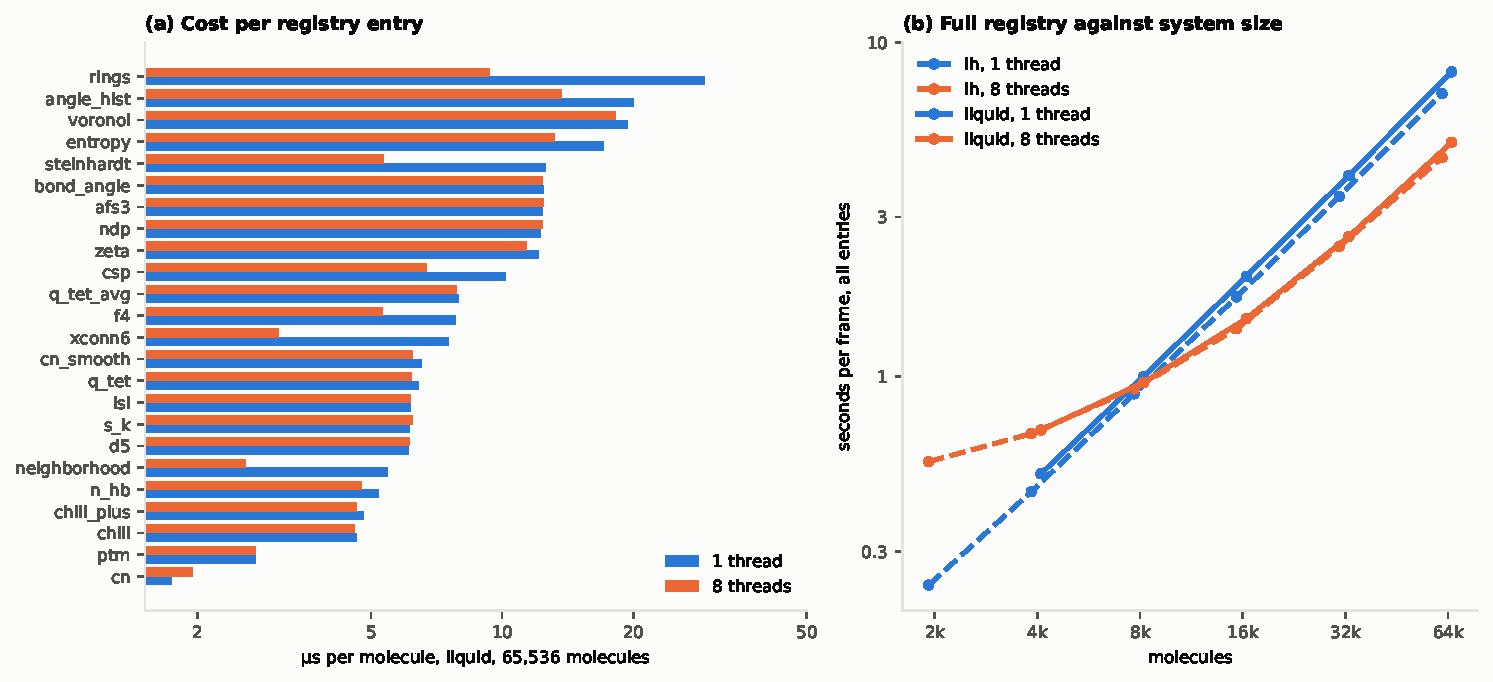
\includegraphics[width=\linewidth]{../benchmarks/results/figures/F6_cost.pdf}
\caption{Computational cost on an Intel Core i7-12700F, median of three warm
repeats, each from a fresh snapshot (neighbor search included). (a) Time per
molecule for each registry entry, liquid with 65,536 molecules, one and eight
threads. (b) Time per frame for all entries against system size; Ih solid,
liquid dashed.}
\label{fig:cost}
\end{figure}

\subsection{What the benchmark does not cover}
\Cref{tab:coverage} defines the boundaries of the benchmark. Within them,
several questions remain open. The sensitivity scan covers one temperature
and the ambient phases only, and varies one factor at a time. Only one
temperature is available for most phases, and one pressure for each
high-pressure phase. Ices IV, IX and XI--XVII and the empty clathrate
frameworks were studied only as ideal structures; amorphous ices were not
studied at all, and no three-site water model was included. Pairwise
separation by one threshold does not establish that a single multiclass
classifier would work for all phases at once. The supercooled liquid references are still aging slowly, and
ideal-crystal results for proton-ordered phases depend on the GenIce cell
geometries. Finally, scoring per molecule does not test a parameter as a CV;
that requires continuity at neighbor exchanges, correct gradients and,
ideally, committor analysis.

%=====================================================================
\section{Practical guide}\label{sec:guide}
%=====================================================================
\Cref{tab:guide} condenses the benchmark into recommendations by task. Five
rules of thumb follow from it.
\begin{enumerate}
\item \emph{Average.} At finite temperature, averaging over the first shell
is worth more than any other design choice. Averaged entropy, $\bar q_6$ and
$\bar Q$ separate ambient ice from liquid at 0.98--1.00; their unaveraged forms
at 0.78--0.85.
\item \emph{Use bond orientations for stacking.} Only averaged low-$l$
Steinhardt parameters, $F_4$ and crystalline connections see the difference
between Ih and Ic in thermal frames; rings and radial parameters do not.
\item \emph{Do not move thresholds of distance- or density-based parameters}
between water models, boxes, protocols or cutoffs without recalibrating them,
and be suspicious of separations found only in quenched frames.
\item \emph{Keep the averaging radius with the threshold.} The first-shell
cutoff barely affects averaged and bond-orientational parameters, but the
averaging radius and the entropy radius change their values and, for
$\bar q_3$, their meaning. Report both and recalibrate when either changes.
\item \emph{Recalibrate for high pressure.} No single parameter separates all
high-pressure ices from liquid at their own pressure; choose by pair, and
compare against liquid at the same pressure.
\end{enumerate}

\begin{table}[H]
\centering
\small
\caption{Recommendations, valid for the conditions of \cref{tab:coverage}:
TIP4P/Ice at 220~K (Ih/Ic also at 250~K) with five independent preparations;
TIP4P/2005 at 220 and 200~K and mW at 220~K with three; six high-pressure
ices and liquids at 0.3--3.0~GPa and 220~K with two; default neighbor
settings unless stated. Rankings are the same for oracle and held-out scores.
In these data, separations below about 0.65 did not reproduce across
preparations.}
\label{tab:guide}
\begin{tabular}{>{\raggedright\arraybackslash}p{.24\linewidth}>{\raggedright\arraybackslash}p{.38\linewidth}>{\raggedright\arraybackslash}p{.28\linewidth}}
\toprule
Question & Best in the benchmark & Avoid \\
\midrule
Ice vs.\ liquid, ambient & $\bar s$, $\bar q_6$, $\bar Q$; six-ring fraction if no
averaging is wanted & CN, $N_\mathrm{HB}$ \\
Ih vs.\ Ic & $\bar q_3$, $\bar q_4$; $F_4$ if hydrogens are available & ring
statistics, unaveraged parameters \\
Polytype labels in nuclei & CHILL+ (Ih, stacking-disordered), CHILL or
CHILL+ (Ic); in constructed seeds at 220~K, polytype recall reaches 90\% only
5--7~\AA{} below the surface, and CHILL+ assigns shallower molecules mostly
to its interfacial class & CHILL for Ih; PTM polytype labels within
${\sim}7$~\AA{} of an interface \\
Distinguishing crystal phases & $\bar s$, smooth CN, Voronoi asphericity,
$\bar Q$; $\bar q_6$ for VII/VIII & $\hat w_4$, $\hat w_6$, $D$, $N_\mathrm{HB}$,
$A_3$ \\
High-pressure ice vs.\ liquid at the same pressure & per pair
(\cref{fig:pressure}): $\bar s$ for III, VI, VII, VIII; six-ring fraction for
II; $\bar q_4$ for V (0.84 at best); no single parameter above 0.69 for all &
ambient-pressure choices without checking \\
Proton-ordered vs.\ disordered & no local parameter tested is reliable
(VII/VIII separate through their oxygen lattices) & -- \\
Oxygen-only models (mW) & $\bar s$, $\bar q_6$, $\bar Q$, $\bar q_3$ (ice vs.\
liquid) and $\bar q_3$, $\bar q_4$ (Ih vs.\ Ic); their TIP4P/Ice thresholds
transferred within 0.01 at 220~K, thermal frames, default settings & thresholds
of distance parameters from other models \\
\bottomrule
\end{tabular}
\end{table}

\subsection{Software}
Most parameters are available in more than one package, but with different
conventions. freud~\cite{Ramasubramani2020} and pyscal~\cite{Menon2019}
compute Steinhardt parameters (including averaged forms) and Voronoi
tessellations; OVITO~\cite{Stukowski2010} provides PTM, identify-diamond,
centrosymmetry and CHILL+; PLUMED~\cite{Tribello2014,PLUMED2019} provides
differentiable versions of coordination and Steinhardt-type parameters, and
with mlcolvar~\cite{Bonati2023} learned CVs;
MDAnalysis~\cite{MichaudAgrawal2011,Gowers2016} handles trajectories and
hydrogen-bond analysis; DScribe~\cite{Himanen2020} computes high-dimensional
descriptors. SolOrder, used here, implements all parameters of
\cref{tab:taxonomy} on MDAnalysis universes with parallel, Numba-compiled
kernels, and wraps SOAP, ACSF and MBTR through DScribe. Its thread
parallelism pays off only for a few parameters (\cref{sec:cost}). It is an analysis
library: none of its parameters provides gradients, so CVs should be taken
from PLUMED. Packages differ in neighbor rules, normalization and the
averaging of $q_{lm}$ vectors versus scalars; agreement between them should
be checked, not assumed.

\subsection{Reproducibility checklist}
When reporting results that depend on a local order parameter, state:
\begin{enumerate}
\item the exact definition and the code and version used;
\item the neighbor rule (cutoff, number of neighbors or Voronoi), the
averaging neighborhood, and whether hydrogens are used;
\item the water model and state point, and where that state point lies on
the model's own phase diagram;
\item the threshold, how it was calibrated (on which reference populations,
thermal or quenched), and whether it was tested on held-out data;
\item for labelers, the classes reported (including interfacial classes) and
how clusters are built from labels;
\item for CVs, how continuity and gradients were checked.
\end{enumerate}

%=====================================================================
\section{Outlook}\label{sec:outlook}
%=====================================================================
Four problems stand out. First, proton order. No local parameter we tested
separates proton-ordered from proton-disordered forms of one oxygen
framework, and those that seem to do so use the accompanying lattice
distortion. Polarization and longer-range orientational correlations remain
to be tested as local observables. Second, interfaces. Every labeler we
tested needs several \AA ngstr\"oms of crystal before it assigns a molecule
its bulk polytype, and labelers differ in what they call the remaining
near-surface molecules, which makes the size of small nuclei and the width of
interfaces depend on the labeler. A benchmark with ground truth at interfaces, for example from
constructed seeds of many sizes, would test learned classifiers where they
are needed. Third, transferability. Thresholds of averaged and
bond-orientational parameters move between water models; thresholds of
distance-based parameters do not, and learned models trained on one model
should be tested on others, including machine-learned potentials of
first-principles quality. Fourth, collective variables. Good per-molecule
separation does not make a good CV; parameters need smooth neighbor
membership and verified gradients, and their quality as reaction coordinates
should be judged by committor analysis rather than by separation of the
end states. Amorphous ices, dense liquids at high pressure and confined water
are the natural next datasets.

\section*{Data and code availability}
SolOrder (version 1.1.0, MIT license), the benchmark scripts, settings
registry and result tables are available in the SolOrder repository. The
figures in \cref{sec:benchmark} are generated by
\texttt{benchmarks/figures.py} from the CSV files in
\texttt{benchmarks/results}.

\bibliographystyle{unsrt}
\bibliography{review}

\end{document}
